\documentclass[11pt,reqno]{amsart}
\usepackage{amsmath,amssymb,amsthm}
\usepackage[margin=1.1in]{geometry}
\usepackage{graphicx}
\usepackage{hyperref}
\hypersetup{colorlinks=true,linkcolor=blue,citecolor=blue,urlcolor=blue}

\theoremstyle{plain}
\newtheorem{theorem}{Theorem}
\newtheorem{lemma}[theorem]{Lemma}
\newtheorem{corollary}[theorem]{Corollary}
\newtheorem{proposition}[theorem]{Proposition}
\theoremstyle{definition}
\newtheorem{remark}[theorem]{Remark}
\newtheorem{conjecture}[theorem]{Conjecture}
\newtheorem{definition}[theorem]{Definition}

\newcommand{\R}{\mathbb{R}}
\newcommand{\Z}{\mathbb{Z}}
\newcommand{\Q}{\mathbb{Q}}
\newcommand{\N}{\mathbb{N}}
\DeclareMathOperator{\Area}{Area}

\title[A signed-direction invariant for triangle tilings]{A signed-direction invariant for triangle tilings, and the exclusion of primes congruent to $3$ modulo $4$}
\author{Vico Bonfioli}
\date{\today}

\begin{document}

\begin{abstract}
For a triangle $T$ and a triangle $ABC$, an \emph{$N$-tiling} is a dissection of $ABC$ into $N$
triangles each congruent to $T$. Erd\H{o}s asked which $N$ occur; a folklore conjecture is that no
prime $N\equiv 3\pmod 4$ with $N>3$ does (the value $N=3$ occurs). By the classification of
Laczkovich and the branch theorems of Beeson, the conjecture reduces to a tile with a $2\pi/3$ angle
on a non-equilateral triangle, where a prime count forces $ABC$ isosceles. For that isosceles case
Beeson ruled out $N<36$ and explicitly left open whether $N$ can be prime (the smallest \emph{known}
tiling has $2673$ tiles); we settle it. We introduce a translation-invariant, signed-direction
tiling functional, linear in edge length and hence insensitive to non-edge-to-edge incidences, whose
integrality forces, for an isosceles target, that $(c-a-b)/\sqrt b$ be an integer for a primitive
triple with $c^2=a^2+ab+b^2$; an elementary lemma shows this never occurs. With a self-contained
reduction of the scalene shapes, and with the base-$\beta$ branch excluded by the forcing chain of
the companion note, this excludes every prime $\equiv 3\pmod 4$ exceeding $3$
\emph{except} the base-$\beta$ candidates $N=3f^2-e^2$, conditional on the cited classification of
the remaining branches. Those candidates are exactly the primes $\equiv11\pmod{12}$
(Theorem~\ref{thm:mod12}), so the exclusion is unconditional on the class $7\pmod{12}$ --- half of
all primes $\equiv3\pmod4$ by Dirichlet, and the class containing $19$. The class $11\pmod{12}$
remains open in general; its members are settled individually by exact search, and $42$ of them lie
below $1000$, of which six are so far resolved. Beyond primes, we determine the admissible spectrum of each sporadic $2\pi/3$
branch --- for the isosceles target, writing $b=de^2$ with $d$ squarefree, every count has the form
$N=dw^2(a+2b)$ with $e\mid w(c-a-b)$ --- bounding the realizable set from outside; and a
spectrum theorem shows that the counts passing all invariant conditions on the isosceles and
$F_1$ targets are \emph{exactly} Zhang's constructed families, closing the necessary side of
those branches; the equilateral criteria likewise reduce to elementary divisor conditions. Combining the spectra with the published
branch theorems and an exhaustive exact search of the surviving finite instances, we settle every
previously undetermined value up to $80$: no triangle can be cut into $14$, $15$, $21$, $22$, $30$,
$33$, $35$, $38$, $39$, $42$, $51$, $55$, $56$, $57$, $60$, $69$, or $76$ congruent triangles
($46$, $62$, $78$ likewise, and $79$ --- a prime --- by the main theorem); triangles \emph{can} be cut
into $44$, $63$ (a kernel-certified tiling of the scalene $(2\alpha,\beta,\alpha{+}\beta)$ target
$(21,24,18)$, correcting an exclusion asserted in an earlier version of this paper), $77$ (by
Beeson's four-component construction), and $80$ (a sum of two squares) congruent
triangles; the values $66$ and $70$, previously excluded via theorems of \cite{BeesonIII} whose
proofs we show to be unsound, are re-excluded here by direct exhaustive search of their single
surviving instances, so that every $N\le80$ is determined. The same method carries the determined
initial segment past $80$: $86$ and $87$ are excluded here (the latter by exhausting both of its
surviving instances), and $81$, $82$, $85$, $89$, $90$ are realizable, leaving $84$ and $88$ under
search and $83$ excluded only conditionally --- it is the first value whose exclusion depends on the
base-$\beta$ branch hypothesis rather than on an $N$-form, a prime congruence, or an exhaustion. Two of those instances come from branches too sparse to be caught by
$N$-forms: the isosceles base-$\alpha$ shape, which has just three instances in all of $N\le90$, and
the scalene $2\pi/3$ shape $F_4$, whose minimal count is exactly $88$. The $44$-tiling is exhibited explicitly --- the isosceles $(16,16,22)$
cut into $44$ copies of the $(2,3,4)$ tile, found by search and verified exactly, to our
knowledge the first tiling in the isosceles $3\alpha+2\beta=\pi$ cases and the smallest known
tiling in any incommensurable branch. A collar induction driven by a kernel-verified $22$-tile
parallelogram certificate realizes $N=11m^2$ for every $m\ge2$, and with the branch exclusion at
$m=1$ the instance spectrum of this (target, tile) pair is completely determined: tileable if and
only if $m\ne1$, apparently the first incommensurable pair with no undecided instance. A second
complete pair over the same tile follows from the cevian decomposition: the scalene
$(2\alpha,\beta,\alpha{+}\beta)$ target realizes $N=7m^2$ exactly for $m\ge2$, contributing
$175$. The phenomenon does not persist along the family. For the next member the scale-$2$ target admits no
tiling at all ($N=104$ on the tile $(3,8,9)$, by exhaustive search), so the unit parallelogram is
constructible for every member of that family while the seeds of the induction are not, and the
instance spectrum depends on the member rather than following a single law. Membership in the
tile-count set is shown to be decidable. The arithmetic and combinatorial layer is
machine-checked in Lean~4 with Mathlib.
\end{abstract}

\maketitle

\section{Introduction}

Let $T$ be a triangle (the \emph{tile}). An \emph{$N$-tiling} of a triangle $ABC$ is a way of
writing $ABC$ as a union of $N$ triangles, each congruent to $T$, with pairwise disjoint interiors.
We do \emph{not} assume the tiling is edge-to-edge: a vertex of one tile may lie in the relative
interior of an edge of another. Erd\H{o}s asked (reported by Soifer~\cite{Soifer}) to determine the
set of $N$ for which some triangle admits an $N$-tiling by some tile. Every perfect square occurs
(any triangle, by the $n^2$ subdivision), and Soifer observed that $n^2+m^2$, $2n^2$, $3n^2$ and
$6n^2$ occur as well; in particular $3=3\cdot 1^2$ occurs. The outstanding question is whether the
primes $\equiv 3\pmod 4$ that exceed $3$, which are exactly the odd primes that are neither sums of
two squares nor of the form $3n^2$, are excluded.

\begin{theorem}\label{thm:main}
Let $N>3$ be a prime with $N\equiv 3\pmod 4$ which is \emph{not} a base-$\beta$ candidate --- that is,
$N\ne 3f^2-e^2$ for every coprime pair $1\le e<f$. Then $N$ is not a number of congruent triangles
into which some triangle can be cut. In particular, since $19$ is not of that form, no triangle can be
cut into $19$ congruent triangles.
\end{theorem}

\begin{theorem}[Full prime exclusion, conditional]\label{thm:fullprime}
Assume the complete-corner-wall hypothesis of the companion note \cite[Hyp.~5.1]{Companion}. Then no
prime $N\equiv 3\pmod 4$ with $N>3$ is a number of congruent triangles into which some triangle can
be cut.
\end{theorem}
\begin{proof}
By Theorem~\ref{thm:main} and Theorem~\ref{thm:mod12} it remains to exclude the base-$\beta$
instances, i.e.\ the primes $\equiv 11\pmod{12}$, at $m=1$ for each representation $(e,f)$. Under the
stated hypothesis this is the base-$\beta$ branch theorem of the companion note \cite{Companion}. The
argument there is a finite forcing chain (walk trichotomy; corner, partner and strip forcing; the
surplus lattice; the column--filler recursion with its orientation congruences; the feet budget; the
$T_{\mathrm{mid}}$ corner kill and the pentagon lemma), with the arithmetic components kernel-checked
in Lean and the smallest members additionally settled by certified exhaustive refutations. Each
representation of a prime is a separate instance and each is excluded.
\end{proof}

\begin{remark}[What is unconditional, and what is not]\label{rem:conditional}
The hypothesis in Theorem~\ref{thm:fullprime} is not cosmetic and we flag it plainly. It asserts that
in a base-$\beta$ tiling neither base corner is starved or broken, so that each corner block is a
complete wall of whole $b$-edges. The companion's funnels and its pentagon lemma both consume it, and
the companion itself identifies the same statement --- that the mismatch segment reaches the base ---
as the highest-value open step of the branch. It is not a formalization debt: it is an unwritten
mathematical step, and until it is supplied, the folklore conjecture is not resolved here.

Unconditionally, this paper proves: no prime $N\equiv7\pmod{12}$ is a tile count (such $N$ are not
base-$\beta$ candidates at all, by Theorem~\ref{thm:mod12}, so Theorem~\ref{thm:main} applies with no
exception) --- in particular $N=19$; and the individual exclusions
$N=11,23,26,47,59,66,71,107$, each by a certified exhaustive search of every surviving instance,
which depend on no branch theorem whatever. The class $11\pmod{12}$ beyond those values, $N=83$
first among them, is \emph{not} settled unconditionally.

That the hypothesis collapses at $e=1$ is recorded in the companion, whose Remark on the side
parameter ends: complete blocks make the base read $a^fbc$, ending in a $c$-edge, while its
reduction theorem forces $a$-edges at both ends, so ``Hypothesis (walls) is thus not a step towards
the $e=1$ case; at $e=1$ it \emph{is} the case.'' We restate it because its consequences for the
present theorem were not drawn: at those members the hypothesis is equivalent to its own conclusion,
so Theorem~\ref{thm:fullprime} carries no $e=1$ content beyond the vacuous.

Two things are added here. First, the clash can be located at the \emph{west} corner alone. A
complete west block has $f$ $a$-feet, consecutive and starting at the corner, so it asks the base
word to begin with $a^f$; with exactly $f$ letters $a$ available and a final $a$ forced, that is
$f+1$ of them. The companion's own argument invokes the east corner's $c$-foot, and a separate
remark, finding the same incompatibility there, retreats to a west-only reading of the hypothesis as
``$p=0$''. That retreat is not available: the west is precisely where the west-only argument fails,
and the west block is the sole premise the derivation of $p=0$ ever had. Second, the failure is
sharply confined to $e=1$, as the next paragraph shows. Both are formalised in
\texttt{lean/Erdos634/WallsCircular.lean} (\texttt{west\_block\_never\_complete},
\texttt{walls\_b\_hits\_tail\_iff\_e\_one}), axiom-clean.

No progress is lost to this. The $e=1$ members were never reached through the hypothesis in any
case: both routes to them --- the companion's forcing chain and our own assembly
(\texttt{lean/Erdos634/E1Assembly.lean}) --- run to the same single geometric fact, that the
multiples of $f$ in $[0,f^2)$ are tiling vertices on the base, and neither invokes the hypothesis at
any point. What is lost is only the appearance that the hypothesis was doing work at $e=1$; the real
state of the subfamily is a reduction to that one fact, not a closure. Something is also gained.
The hypothesis is precisely the assertion that the corner growth \emph{completes} rather than
breaks, so knowing that it never holds removes the completion branch from the companion's case split
at $e=1$: both corners break, at most one break is on the base because the walk carries a single
$c$, and therefore some corner breaks on a side. The forced column of $f$ tiles is then present in
every tiling of every $e=1$ member rather than in one branch of an alternative.

The same step corrects what the open question at $e=1$ was taken to be. The companion identifies it
as the single statement ``$p=0$'', the assertion that an equal side carries no $a$-edge. That is
now refutable: a corner block breaks on a side by failing to read a $c$ where it demands one, and its
partial far side lies on the adjacent equal side, so \emph{at least one equal side carries an
$a$-edge} in every tiling of every $e=1$ member. Read symmetrically, as the companion reads it,
$p\ge1$. Both of that identification's supports fail independently as well --- the derivation of
$p=0$ runs through the complete west block, and its claimed sufficiency substitutes complete blocks
for $p=0$, which needs a converse stated only inside a conjecture proved at $f=2,3,4$. What survives
as the open step is the cascade rather than the parameter: whether the chain from such an $a$-edge
terminates in a collision. Its premise is now discharged rather than hypothetical. (The prime candidates in the subfamily all have $f$ even, since $3f^2-1$ is even for odd $f$
--- \texttt{lean/Erdos634/ThinHole.lean}, \texttt{f\_even\_of\_prime}, where the consequence
that an argument biting only on odd $f$ is irrelevant to the primes is already recorded.) The failure at $e=1$ is in fact twofold, the second
kill being independent of the companion's reduction theorem altogether. The hypothesis pins the base word
to $a^fb^ec^e$; its length is $f+2e$, its $b$'s occupy positions $f+1,\dots,f+e$, and
Proposition~\ref{prop:cornerpara} forbids a $b$ in the last two positions, which begin at $f+2e-1$.
A $b$ reaches them exactly when $f+e\ge f+2e-1$, that is exactly when $e=1$ --- and then the word is
$a^fbc$, whose $b$ sits in the penultimate slot.

That computation also shows why the collapse does not propagate. At $e\ge2$ the $b$-block clears the
forbidden tail by $e-1$ slots, being separated from it by the $e$ $c$-feet of the east block; only at
$e=1$ does that block shrink to a single foot and let the $b$ touch the tail. We have tested the
walls word against the rest of what is proved at $e\ge2$ --- the walk counts $(f,e,e)$ at a
separated thick member, which it realises; Proposition~\ref{prop:cornerpara}, which it satisfies;
and the $e=1$ argument that the base ends with an $a$, which runs on the uniqueness of the single
$c$ and is unavailable --- and found no clash. Hypothesis (walls) is a genuine positional
strengthening at $e\ge2$, and Theorem~\ref{thm:fullprime} retains its content on that residue,
which is where the prime problem now lives.
\end{remark}

\begin{theorem}[The exceptional set is a congruence class]\label{thm:mod12}
Let $p>3$ be prime with $p=3f^2-e^2$ for some coprime $e,f$. Then $p\equiv11\pmod{12}$. Conversely
every prime $p\equiv11\pmod{12}$ is of that form. Hence the base-$\beta$ candidates among the primes
are exactly the primes $\equiv11\pmod{12}$.
The forward direction is machine-checked
(\texttt{lean/Mod12.lean}, \texttt{base\_beta\_prime\_mod12}), axiom-free beyond \texttt{propext},
\texttt{Classical.choice} and \texttt{Quot.sound}; it is the direction that makes the class
$7\pmod{12}$ unconditional. The converse uses quadratic reciprocity and the class group of
discriminant $12$ and is not formalised.
\end{theorem}

\begin{proof}
($\Rightarrow$) If $3\mid e$ then $3\mid p$, impossible for a prime $p>3$; so $e^2\equiv1\pmod 3$ and
$p\equiv-1\equiv2\pmod3$. Next, $e,f$ are not both even (coprimality) and not both odd, since then
$p=3f^2-e^2\equiv3-1=2\pmod4$ would be an even prime exceeding $3$; in either remaining case
$p\equiv3\pmod4$. Combining, $p\equiv11\pmod{12}$.
($\Leftarrow$) For $p\equiv11\pmod{12}$ we have $p\equiv3\pmod4$ and $p\equiv2\pmod3$, so by
reciprocity $\left(\frac3p\right)=1$ and $p$ splits in $\Q(\sqrt3)$. The discriminant-$12$ form class
group has order two, represented by $x^2-3y^2$ and $3y^2-x^2$; the first forces $p\equiv1\pmod3$ and
the second $p\equiv2\pmod3$, so $p$ is represented by $3y^2-x^2$. Primitivity is automatic for
prime $p$.
\end{proof}

\begin{theorem}[The first complete member]\label{thm:realize12}
Let the tile be $(2,3,4)$ and the target the isosceles triangle with base angles $\beta$
(the base-$\beta$ member $(e,f)=(1,2)$, instances $N=11m^2$). Then the instance is tileable if and
only if $m\ne1$: every $N=11m^2$ with $m\ge2$ is realized, and $N=11$ is excluded. This is, to our
knowledge, the first (target, tile) pair with incommensurable angles whose instance spectrum is
completely determined.
\end{theorem}
\begin{proof}
Exclusion at $m=1$ is the base-$\beta$ branch theorem \cite{Companion}. Realizability is the collar
induction of the companion note: the collar of $\Delta_m$ (the bottom two rows of the $m$-fold cell
subdivision) decomposes into $m-2$ sheared parallelogram columns and one scale-$2$ corner triangle,
all interfaces full straight segments; each column is two translates of the unit parallelogram. The
three seeds are found by exhaustive search and kernel-verified with exact $\Z[\sqrt{15}]$
arithmetic and zero axioms (\texttt{Tiling44.lean}, \texttt{Tiling99.lean},
\texttt{PgramTiling22.lean}: congruence, containment, an explicit separating line per tile pair,
and the exact area identity), and the two-step induction from bases $m=2,3$ is itself
kernel-checked (\texttt{Collar.lean}). See the companion note \cite{Companion} for the full
statement and proof.
\end{proof}

\begin{remark}[The spectrum is member-dependent]\label{rem:memberdep}
Recorded in \cite{Obstructions}.
\end{remark}

\begin{corollary}[Theorem~\ref{thm:main}, congruence form]\label{cor:mod12}
No prime $p\equiv7\pmod{12}$ is a number of congruent triangles into which a triangle can be cut.
Equivalently: a prime $p>3$ with $p\equiv3\pmod4$ is excluded unconditionally unless
$p\equiv11\pmod{12}$.
\end{corollary}

\begin{proof}
A prime $p>3$ with $p\equiv3\pmod4$ satisfies $p\equiv7$ or $p\equiv11\pmod{12}$, the class
$3\pmod{12}$ forcing $3\mid p$. If $p\equiv7\pmod{12}$ then by Theorem~\ref{thm:mod12} it is not a
base-$\beta$ candidate, so Theorem~\ref{thm:main} applies with no exception.
\end{proof}

\begin{remark}[Why the forms, and what the reformulation buys]\label{rem:forms}
Recorded in \cite{Obstructions}.
\end{remark}

\begin{remark}[The quoted form of {\cite[Lem.~6]{BeesonIII}} is false]\label{rem:lem6false}
That lemma is usually quoted as ``every side of $ABC$ carries at least two $c$-edges''. In that form
it is false. Take the tile $(2,3,4)$ and let $ABC=(4,6,8)$, its double; the four-fold midpoint
subdivision is a genuine tiling by four congruent copies, and its sides decompose as $b^2$, $c^2$,
$a^2$ --- two of the three carry \emph{no} $c$-edge. Here $ABC$ is similar to the tile, a case treated
separately in \cite{BeesonIII}, so the true statement must carry hypotheses that the usual quotation
omits. We therefore do not use it: Proposition~\ref{prop:b3prime} now invokes only the $\gamma$-trap
(at least \emph{one} $c$-edge per side), which is proved here from the vertex figures and
machine-checked, and which suffices because the base length identity gives $Y\le(g-M)b$
unconditionally --- a single $c$-edge already contradicts. An exhaustive check over all
$11{,}338$ admissible pairs $(N,M)$ with $N<2500$ prime found \emph{no} decomposition of the base
containing even one $c$-edge, so the margin is not delicate; the citation
\cite[Lem.~45(iii)]{BeesonIII} is likewise not needed for the conclusion.
\end{remark}

\begin{remark}[The scope of Theorem~\ref{thm:main}]\label{rem:mainscope}
The base-$\beta$ exception is essential. The base-$\beta$ candidates are exactly the $N=3f^2-e^2$ with
$\gcd(e,f)=1$, $1\le e<f$. Those with $e,f$ of opposite parity are $\equiv3\pmod4$; those with $e,f$
both odd are $\equiv2\pmod4$, hence even, so among the \emph{primes} only the former occur --- and by
Theorem~\ref{thm:mod12} they are exactly the primes $\equiv11\pmod{12}$. (Composite candidates of
either parity occur and appear in Table~\ref{tab:basebeta}: $26$, $66$ and $74$ are $\equiv2\pmod4$.)
The smallest prime candidates are
\[ 11,\ 23,\ 47,\ 59,\ 71,\ 83,\ 107,\ 131,\ 167,\ 179,\ 191,\ \dots \]
For each, the tile $(ef,\,f^2-e^2,\,f^2)$ and the target $(f^3,f^3,e(3f^2-e^2))$ pass every
\emph{sound} necessary condition (Remark~\ref{rem:isobeta}); the only published exclusion is
\cite[Thm.~14]{BeesonIII}, whose $g\mid M$ is not merely unproven but \textbf{false}
(Remark~\ref{rem:thm14false}), so we cannot invoke it, and no general replacement is known \cite{Companion}. The theorem therefore cannot drop the exception without appealing to that
false citation. The candidates are settled one at a time by exhaustive search
(Table~\ref{tab:basebeta}): $11,23,47,59,71,107$ are excluded and $83$ remains under search. Thus
Theorem~\ref{thm:main} is unconditional for every prime
$N\equiv3\pmod4$, $N>3$, outside the sequence above, and for $11,23,47,71,107$ besides. The
principal consequence is unaffected: $19\ne3f^2-e^2$, and the two frontier claims of
Section~\ref{sec:full} rest only on candidates that have been searched.
\end{remark}

\noindent The restriction $N>3$ is necessary: an equilateral triangle joined to its centre splits
into $3$ congruent triangles, so $N=3$ occurs.

The proof rests on Laczkovich's classification of triangle tilings~\cite{Laczkovich1995,
Laczkovich2012}, organized by Beeson across a series of papers \cite{BeesonI, BeesonIII,
BeesonIso, BeesonSeven, BeesonEq}. For a prime number of tiles every branch of the classification
is excluded by an existing theorem, with one exception: a tile having a $2\pi/3$ angle, tiling a
non-equilateral triangle. We treat that branch.

Zhang~\cite{Zhang} classifies the non-equilateral
$2\pi/3$ shapes into six sporadic similarity types (Section~\ref{sub:shapes} below), constructs
families of tilings for each, and conjectures that the constructed $N$, all composite, are the only
ones; the present results prove the no-prime half of that conjecture for the isosceles type, and
reduce the scalene types directly. For the isosceles type Beeson~\cite{BeesonIso} proved that no
tiling exists with $N<36$ and \emph{explicitly left open whether $N$ can be prime}; the smallest
tiling presently known has $2673$ tiles (Herdt, reported in~\cite{BeesonIso}). The invariant below
settles the question, excluding \emph{every} prime. The adjacent Erd\H{o}s Problem~633, on tilings
into a square number of triangles, was recently settled by Beeson, Laczkovich and
Zhang~\cite{Erdos633}.

Two reductions prepare it. First, such a tile has commensurable sides, so after scaling we may take
it integer-sided with $c^2=a^2+ab+b^2$; for the \emph{isosceles} targets to which the theorem
reduces, this is Beeson's \emph{accepted} isosceles paper (\cite[Thm.~12.5]{BeesonIso}: any
isosceles triangle tiled by a $2\pi/3$-tile with $\alpha/\pi$ irrational forces the tile rational),
so that citation covers the isosceles targets; but the reduction to an isosceles
target (Section~\ref{sec:reduction}) already works with an integer-sided tile, so the rationality
input actually used in that order is the general-target theorem of Beeson--Zhang, a preprint --- we
record this plainly rather than claim a refereed input; the general-tile rationality of
Beeson--Zhang~\cite{BeesonZhang} gives the same uniformly. Second, an elementary
area-and-incidence argument shows that a \emph{prime} number of such tiles forces $ABC$ to be
\emph{isosceles} (Section~\ref{sec:reduction}).

The main construction is in Section~\ref{sec:invariant}. The natural parity argument for a $2\pi/3$
tile (a black/white colouring of the tiles) fails, because a vertex of the tiling may be surrounded
by an even number of tiles, so no consistent two-colouring exists. We replace it by a functional
$\Phi$ that assigns to a directed edge of direction $\theta=j\frac\pi3+k\alpha$ the weight
$(\text{length})\cdot(-1)^j$. Two features make it work: $\Phi(\theta+\pi)=-\Phi(\theta)$, so
interior edges cancel; and the weight is \emph{linear in edge length}, so the cancellation is
unaffected by non-edge-to-edge incidences, where one long edge meets several shorter ones summing
to it. Summing over the tiles, $\Phi$ of the boundary equals an integer multiple of a fixed
tile-value $c+a-b$. For an isosceles target this forces $(c-a-b)/\sqrt b\in\Z$, which never holds
(Section~\ref{sec:isosceles}). Assembling the branches proves Theorem~\ref{thm:main}
(Section~\ref{sec:assembly}).

The combinatorial claims are verified by the scripts in the accompanying repository, and the entire
arithmetic layer, including Lemma~\ref{lem:nonint} and the reduction of Section~\ref{sec:reduction},
is formalized and machine-checked in Lean~4 with Mathlib; see Section~\ref{sec:verification}.

\section{Preliminaries}\label{sec:prelim}

\subsection*{The classification.}
Fix a prime $N=p>3$ with $p\equiv 3\pmod 4$. By Laczkovich~\cite{Laczkovich1995,Laczkovich2012},
every $N$-tiling of a triangle falls into one of finitely many types of pairs $(ABC,T)$. The
relevant dichotomy, in Beeson's organization~\cite{BeesonSeven}, is: either the angles of $T$ are
pairwise commensurable with $\pi$, or they are not. If they are commensurable, then $N$ is a square,
a sum of two squares, or $2$, $3$ or $6$ times a square \cite[Thm.~3 and Table~3]{BeesonSeven}; but
$p>3$ with $p\equiv3\pmod4$ is a square only if $p$ is one (it is not), a sum of two squares only if
$p\not\equiv3\pmod4$, and $2n^2,3n^2,6n^2$ only if $p$ is even or $3\mid p$ (here $p$ is odd and
$p>3$), so $p$ is none of these (it is precisely for $p=3=3\cdot1^2$ that this step would fail).
If the angles are not commensurable, then, after the right-angle and similar-tile cases, which give
$N$ a sum of two squares or $N=n^2$ \cite{BeesonI, SWW}, the tile has a special angle and falls into
one of: $3\alpha+2\beta=\pi$, for which $N$ is not prime (originally \cite{BeesonIII}; see
Remark~\ref{rem:b3prime} and Propositions~\ref{prop:b3prime} and~\ref{prop:isoalphaprime} ---
the arithmetic core is machine-checked in Lean for \emph{four} of the five target shapes, with our
own proofs replacing Beeson's Theorems~18 and~20, whose printed arguments are unsound; the fifth,
the base-$\beta$ isosceles target, is the exception, treated in
Remark~\ref{rem:isobeta}); an isosceles tile with
$\gamma=2\alpha$, for which $N$ is not squarefree \cite[Thm.~11.7]{BeesonIso}; or the tile has an
angle equal to $\pi/3$ or $2\pi/3$. The case of a $\pi/3$ or $2\pi/3$ tile on an \emph{equilateral}
triangle gives $N$ not prime \cite{BeesonEq}. What remains for a prime $N$ is a tile with a $\pi/3$
or $2\pi/3$ angle on a \emph{non-equilateral} triangle. The vertex enumeration of
Section~\ref{sub:shapes} shows the $\pi/3$ case admits only equilateral or tile-similar $ABC$,
already covered; so the sole remaining branch is a $2\pi/3$ tile, which we now fix.

\begin{remark}[The $3\alpha+2\beta=\pi$ prime exclusion]\label{rem:b3prime}
The step above invokes \cite{BeesonIII} for the claim that a $3\alpha+2\beta=\pi$ tiling has $N$
composite. For the two scalene targets $(2\alpha,\beta,\alpha{+}\beta)$ and $(2\alpha,\alpha,2\beta)$
this is Beeson's Theorems~8 and~12, whose arithmetic cores we machine-check in Lean
(\texttt{lean/Beeson3NotPrime.lean}): the first tiling equation $N+M^2=2K^2$ with $K\mid N$ admits no
odd prime, and the second forces $N=(2f^2-e^2)(3f^2-e^2)k^2$ --- a product of two factors exceeding
$1$, hence composite. The isosceles target with base angles $\alpha{+}\beta$ is
Beeson's Theorem~18, but its published proof is \emph{unsound}: under Beeson's scaling
$a=N-M^2,\ c=N+M^2,\ b=c-a^2/c$ one has $bc=c^2-a^2=4NM^2$, so $c^2b=4NM^2(N+M^2)\equiv0\pmod N$
\emph{identically} (no primality used), not the $M^4(M^2+1)$ his argument needs --- a dropped factor
of $a$; the residue is already false on genuine composite tilings ($N=48,\,M=4$ gives $c^2b\equiv0$
while $M^4(M^2+1)\equiv32$), so the step forcing $N=M^2+1$ is vacuous. The conclusion is nonetheless
correct, by the base-length obstruction of Proposition~\ref{prop:b3prime}.

Two further defects of \cite{BeesonIII} affect the base-$\alpha$ target. First, the squarefree
assertion of its Lemma~8 (``$g=\gcd(a,c)$ is squarefree'') is \emph{false}: the tile $(4,15,16)$
--- a genuine $3\alpha+2\beta$ tile, $e=1$, $f=4$ --- has $g=4$ (its proof breaks at the inference
$p^2\mid a\Rightarrow p^2\mid\hat a$); the parametrized family $(ef,\,f^2-e^2,\,f^2)$ realizes
\emph{every} $f$ coprime to $e$, squarefree or not. Second, Theorem~19's claim $g\mid M$ rests on
that lemma \emph{and} on the assertion that $bc^3(a+c)$ is not divisible by $g^5$ --- but with
$c=g^2$ it carries $g^7$ identically, so the argument collapses, and with it the proof of the
base-$\alpha$ prime exclusion (Theorem~20). Proposition~\ref{prop:isoalphaprime} repairs the
latter without any appeal to $g\mid M$.
\end{remark}

\begin{proposition}[Base-$\alpha$ prime exclusion, replacing {\cite[Thm.~20]{BeesonIII}}]\label{prop:isoalphaprime}
No isosceles triangle with base angles $\alpha$, where $3\alpha+2\beta=\pi$ and
$\alpha\notin\Q\pi$, is $N$-tiled for $N$ prime.
\end{proposition}

\begin{proof}
Write $s=e/f$ in lowest terms, so the tile is $(ef,\,f^2-e^2,\,f^2)$. Two necessary conditions
suffice: the tiling equation $N(f-e)(2f+e)^2=M^2(f+e)(2f^2-e^2)$ (the sound half of
\cite[Thm.~19]{BeesonIII}) and the integrality of the equal side $X$, where
$X^2=Nbc/(2-s^2)$. Substituting the tiling equation into $X^2$ gives the exact value
$X=M(f+e)f^2/(2f+e)$; as $\gcd(2f+e,f)=\gcd(2f+e,f+e)=1$, integrality forces $(2f+e)\mid M$.
Writing $M=(2f+e)m$ reduces the tiling equation to
\[
N(f-e)\;=\;m^2\,(f+e)\,(2f^2-e^2).
\]
Put $d=f-e$ and $Q=2f^2-e^2=e^2+4ed+2d^2$. Then $\gcd(d,Q)=1$ (a common prime would divide $e^2$,
hence $e$, hence $\gcd(e,f)$), so the minimal prime factor of $Q\ge7$ divides $N$ and equals $N$;
writing $Q=NQ_1$ and cancelling $N$ leaves $d=m^2(f+e)Q_1\ge f+e>f-e=d$, a contradiction. Both
arithmetic pillars are machine-checked in Lean (\texttt{lean/IsoAlphaPrime.lean}, axiom-clean:
\texttt{isoalpha\_X\_forces}, \texttt{isoalpha\_not\_prime}).
\end{proof}

\begin{remark}[The base-$\beta$ target]\label{rem:isobeta}
The fifth target, isosceles with base angles $\beta$, is the one shape where we cannot replace
Beeson's argument with a sound one. Beeson's Theorem~14 also asserts $g\mid M$, by a proof of the
same broken shape as Theorem~19's (it claims $abc^5M^2$ is not divisible by $g^7$, but with $c=g^2$
it carries $g^{11}$). And here the defect \emph{bites}: the sound necessary conditions do not exclude
prime $N$. With $s=e/f$ in lowest terms the tile is $(ef,\,f^2-e^2,\,f^2)$, the equal side is
$X=f^3M/(f+e)$ and the base is $Y=eM(3f^2-e^2)/(f+e)$; integrality of $X$ forces $(f+e)\mid M$, and
writing $M=(f+e)m$ the Theorem-14 equation $N(e+f)^2=M^2(3f^2-e^2)$ collapses to
\[
N=m^2\,(3f^2-e^2),
\]
which \emph{is} prime for $m=1$ and $3f^2-e^2$ prime (e.g.\ $N=11,23,47,59,71,\dots$, always
$\equiv3\pmod4$). Each such $N$ passes every sound necessary condition ($X,Y\in\Z$, parity, range)
and is killed only by the unsound $g\mid M$. Unlike the base-$\alpha$ case
(Proposition~\ref{prop:isoalphaprime}), no arithmetic contradiction follows; \emph{a general proof
that these candidates do not tile is open for $e\ge 2$}, and to our knowledge is not supplied by a
correct argument in the literature.

This last point needs stating explicitly, because the most recent paper in the area asserts the
contrary. Beeson's \emph{No prime tiling of an isosceles triangle} \cite{BeesonNoPrime} (July 2026)
opens with the statement that no isosceles triangle admits a prime tiling, and its Theorem~1 reads:
``Let $T$ be a triangle tiled using a tile $R$ with angles $(\alpha,\beta,\gamma)$ such that
$3\alpha+2\beta=\pi$, and $T$ is not similar to $R$. Then the number of tiles $N$ is not a prime,''
with the proof given in full as ``This is proved in \cite{BeesonIII}, by considering the possible
shapes of $T$ one by one.'' It is a citation, not an independent argument, and \cite{BeesonIII} has
not been revised since v3 of 13 February 2019 --- the text analysed above. Its Theorem~14, which is
verbatim the base-$\beta$ isosceles case, derives
$X^2a(c^2-a^2)(a+c)^2=abc^5M^2$ and then argues that if $g\nmid M$ then $g^6$ divides the right side
but $g^7$ does not. Since that paper's own Lemma~8 gives $c=g^2$, and $g\mid a$, the right side carries
$g^{11}$; the divisibility count is wrong and the contradiction does not follow. We therefore record
that the base-$\beta$ isosceles target remains open in the published record at the time of writing,
and that the present note's contribution --- the $e=1$ family, and the conditional
Theorem~\ref{thm:fullprime} --- addresses a live gap rather than a closed one. For the subfamily $e=1$ the companion note \cite{Companion}
gives a theorem covering every $f\ge2$, whose parity hypothesis was removed at modulus $f$; but its
proof is stated as an architecture with ``the full strip-and-column exposition'' deferred, and the
deferred step is precisely that the forced column \emph{reaches the base}. We do not claim the
$e=1$ family as closed. What is established is a reduction, reached independently twice: the
companion's chain and our own assembly (\texttt{lean/Erdos634/E1Assembly.lean}) both terminate on
the single geometric fact that the multiples of $f$ in $[0,f^2)$ are tiling vertices on the base.
The candidates so reduced are $11, 47, 107, 191, 431,\dots$ --- and, by
Proposition~\ref{prop:repunique} below, that is exactly the set of prime candidates the $e\ge2$
half can never reach --- leaving $e\ge2$ as the open residue on a set disjoint from these. This assessment includes the recent preprint \cite{BeesonNoPrime}
(21~July~2026), which asserts that no isosceles triangle admits a prime tiling: its Theorem~1
disposes of the whole $3\alpha+2\beta=\pi$ branch by citation to \cite{BeesonIII}
(``by considering the possible shapes of $T$ one by one''), and for the present shape the argument
of \cite{BeesonIII} is Theorem~14, refuted above by the $99$-tiling
(Remark~\ref{rem:thm14false}). The genuinely new content of \cite{BeesonNoPrime} is the isosceles
target with a $2\pi/3$-angle tile, proved there by a short-relation argument (its Theorems~8
and~10); that case is Theorem~\ref{thm:iso} of the present paper, obtained here by the
signed-direction functional. The two proofs are independent and the methods are disjoint; the
present proof, together with the repository holding it, was made public on 27~June~2026 and
communicated to the author of \cite{BeesonNoPrime} the same day. For the finitely many instances that bear on the values settled in this
paper we resort to the direct corner-anchored search. An exhaustive audit of $N\le80$ --- computing
the equal side $X$ and base $Y$ exactly and retaining every candidate that passes all \emph{sound}
necessary conditions ($X,Y\in\Z$, parity, range) --- shows the affected set is precisely
\[
\text{primes } \{11,23,47,59,71\}\ \text{(base-}\beta\text{)}\quad\text{and}\quad
\text{composites } \{21,70\}\ \text{(base-}\alpha\text{)},\ \{39,66\}\ \text{(base-}\beta\text{)} .
\]
The engine settles them one at a time; all searches are exact and exhaustive:
\begin{center}
\begin{tabular}{llllr}
$N$ & branch & tile & target & nodes\\ \hline
$11$ & base-$\beta$  & $(2,3,4)$    & $(8,8,11)$      & $135$\\
$21$ & base-$\alpha$ & $(2,3,4)$    & $(12,12,21)$    & $13\,659$\\
$23$ & base-$\beta$  & $(6,5,9)$    & $(27,27,46)$    & $19\,677$\\
$47$ & base-$\beta$  & $(4,15,16)$  & $(64,64,47)$    & $12\,440$\\
$39$ & base-$\beta$  & $(12,7,16)$  & $(64,64,117)$   & $825\,724$\\
$71$ & base-$\beta$  & $(10,21,25)$ & $(125,125,142)$ & $553\,417$\\
\end{tabular}
\end{center}
\noindent each returning \textsc{exhausted, no tiling}. The remaining three --- $N=59$
(base-$\beta$, $(20,9,25)$ on $(125,125,236)$), $N=66$ (base-$\beta$, $(15,16,25)$ on
$(125,125,198)$) and $N=70$ (base-$\alpha$, Remark~\ref{rem:seventy}) --- are still searching, and
their values are treated as pending. For the base-$\beta$ target the
$3\alpha+2\beta$ prime argument rests on either \cite[Thm.~14]{BeesonIII} (whose printed proof is
unsound) or a per-value search, \emph{not} on a machine-checked general theorem; this is the one
remaining gap in the prime dichotomy. The companion note \cite{Companion} removes $N=11$
unconditionally, Remark~\ref{rem:lem6} isolates the $e=1$, $f\ge3$ structure, and
Remark~\ref{rem:nogo} explains why the method \cite{BeesonIII} used cannot repair the rest.
\end{remark}



\begin{remark}[The $e=1$, $f\ge3$ cases are \emph{not} settled]\label{rem:lem6}
For $f\ge3$ the composition $B_1=(a^{f},b,c)$ survives every citation-free constraint above, and it is
then the \emph{unique} possible base. Two consequences follow. First, $B_1$ carries exactly \emph{one} $c$-edge; so \cite[Lem.~6]{BeesonIII} (``every side
carries at least two $c$-edges'') removes it at a stroke --- but that citation is doing \emph{all} of
the work, and any tiling of this family would \emph{refute} Lemma~6 rather than be excluded by it, so
invoking it is tantamount to assuming the conclusion. Given that \cite{BeesonIII} is the source whose
Lemma~8 we show false, whose Theorems~18--20 we show unsound, and whose Theorem~14 we show to be
outright \emph{false} (Remark~\ref{rem:thm14false}), we do not invoke it. Second, our own forcing
argument targets $B_0$, which cannot occur in any case, so it says nothing about $f\ge3$. We
therefore record $N=26,47,74,107,146,191,\dots$ as \emph{open} in this branch, with $N=26,47,74$
independently excluded by exhaustive search.

What survives citation-free is a sharp structure theorem: \emph{if} an $e=1$, $m=1$, $f\ge3$
base-$\beta$ tiling exists, then $q_{\mathrm{equal}}=0$, its base is exactly $(a^{f},b,c)$ with
$E_1=E_k=a$ and the $c$-edge interior, both equal sides begin and end with $c$, and every base
junction is a $(1,1,1)$-vertex.
\end{remark}

The next theorem replaces the $e=1$ case analysis by a classification valid for \emph{every} $e$, and
shows why $m=1$ --- the prime case --- is the rigid one. It is machine-checked
(\texttt{BaseBetaWalks.lean}, axiom-clean).







\begin{proposition}[Unsplittability, and the rigidity of the thick regime]\label{prop:unsplit}
For every coprime $1\le e<f$, neither $a=ef$ nor $b=f^2-e^2$ is a sum of two or more tile edges; and
$c=f^2$ is such a sum if and only if $e=1$, in which case uniquely $c=a^{f}$. Consequently \emph{in the
entire open thick regime, where $e\ge2$, no tile edge splits at all}.
\end{proposition}

\begin{proof}
Reduce $n_a\,ef+n_b(f^2-e^2)+n_c f^2=L$ modulo $f$. For $L=a$: $f\mid n_b e^2$, so $f\mid n_b$ by
$\gcd(e,f)=1$; $n_b\ge f$ overshoots since $fB>ef$ (as $B=f^2-e^2\ge2e+1>e$), so $n_b=0$, and
cancelling $f$ leaves $n_a e+n_c f=e$, forcing $n_c=0$ and $n_a=1$. For $L=b$: $f\mid(n_b-1)e^2$, so
$n_b\equiv1$; $n_b\ge1+f$ overshoots, so $n_b=1$ and the rest vanishes, giving $n_a=n_c=0$. Either way
the total is $1$, never $\ge2$. For $L=c$: $f\mid n_b$ forces $n_b=0$ as before, and $n_a e=f(1-n_c)$
gives $n_c=0$ and $e\mid f$, i.e.\ $e=1$, $n_a=f$.
\end{proof}

\begin{remark}[The golden ratio]\label{rem:golden}
Recorded in \cite{Obstructions}.
\end{remark}



\begin{remark}[Validation on the $44$-tiling]\label{rem:rung2}
Recorded in \cite{Obstructions}.
\end{remark}





\begin{remark}[A parity argument that fails, and why]\label{rem:parityfail}
The $b$-edge pairing argument fails because a longer edge may straddle a $b$-edge rather than abut it, and both genuine tilings contain such straddles. Full discussion in \cite{Obstructions}.
\end{remark}

















\begin{remark}[What the alignment pins, uniformly]\label{rem:align}
Recorded in \cite{Obstructions}.
\end{remark}





\begin{remark}[Why the colouring method cannot close the rest]\label{rem:nogo}
No weighting of directed edges by direction alone can close the remaining branch; the whole class is excluded. Full discussion in \cite{Obstructions}.
\end{remark}

\begin{remark}[Beeson's Theorem~14 is \emph{false}, not merely unsound]\label{rem:thm14false}
The exhaustive engine settles the status of $g\mid M$ outright. The isosceles triangle
$(24,24,33)$ with base angles $\beta$ \emph{is} tiled by $99$ copies of the tile $(2,3,4)$: this is
the base-$\beta$ family at $(e,f,m)=(1,2,3)$, so $X=f^3m=24$, $Y=em(3f^2-e^2)=33$,
$N=m^2(3f^2-e^2)=99$ and $M=(f+e)m=9$. The tiling was found by exact search, re-verified
independently (congruence of all $99$ tiles, disjointness, containment, exact area) against a
separately constructed instance, and is now \emph{machine-verified in Lean~4 with no axioms
whatsoever} (\texttt{lean/Tiling99.lean}: the kernel checks, by pure computation over
$\Z[\sqrt{15}]$ after scaling by $16$, that all $99$ triangles have squared side multiset exactly
$\{1024,2304,4096\}=(16\cdot(2,3,4))^2$, are positively oriented, lie in the closed target
$(384,384,528)=16\cdot(24,24,33)$, admit an explicit separating edge-line for each of the $4851$
pairs, and have signed areas summing exactly to the target's; \texttt{\#print axioms} reports the
theorem depends on no axioms). Since it is this object that refutes \cite[Thm.~14]{BeesonIII},
the refutation now rests on a kernel-checked certificate rather than on a search log.
Its boundary base walk is the multiset $\{a^2,b^7,c^2\}$
($2\cdot2+7\cdot3+2\cdot4=33$), consistent with $q_{\mathrm{base}}\equiv em\equiv1 \pmod 2$.

But $g=\gcd(a,c)=\gcd(2,4)=2$ and $M=9$, so $g\nmid M$. Hence
\[
\textbf{\cite[Thm.~14]{BeesonIII}'s conclusion } g\mid M \textbf{ is FALSE},
\]
not merely unsoundly proved (Remark~\ref{rem:isobeta}); equivalently $f\mid m$ fails, here $2\nmid3$.
Three consequences. (i) The base-$\beta$ prime exclusion cannot rest on Theorem~14 \emph{at all};
only a per-value search remains, which is what we do. (ii) Our own base-$(\alpha{+}\beta)$ and
base-$\alpha$ replacements (Propositions~\ref{prop:b3prime}, \ref{prop:isoalphaprime}) are unaffected:
both were deliberately built to use \emph{no} $g\mid M$. (iii) The values whose exclusion had rested
only on $g\mid M$ ($21,39,66,70$) are demoted (Remarks~\ref{rem:seventy},
\ref{rem:isobeta}); $21$ and $39$ are now excluded by exhaustive search instead. Finally $N=99$ is itself a new realization: $99$
is not a square, a sum of two squares, nor $2n^2,3n^2,6n^2$, so it is not commensurably realizable.
\end{remark}

\begin{proposition}[Dissection basics]\label{prop:dissection}
Let $ABC$ be cut into $N$ triangles $T_1,\dots,T_N$ with pairwise disjoint interiors and union $ABC$.
Then $\sum_i\lvert T_i\rvert=\lvert ABC\rvert$, and if the $T_i$ are pairwise congruent to a tile $T$
then $\lvert ABC\rvert=N\lvert T\rvert$. Moreover, at a point $v\in ABC$ the tiles whose closure
contains $v$ subtend angles summing to $2\pi$ if $v$ is interior to $ABC$, to $\pi$ if $v$ is interior
to a side, and to the corner angle if $v$ is a corner; each summand is a tile angle
$\alpha,\beta,\gamma$ if $v$ is a vertex of that tile, and $\pi$ if $v$ lies in the relative interior
of one of its edges. Hence the sum has the form $p\alpha+q\beta+r\gamma+s\pi$ with $p,q,r,s\ge0$
integers.
\end{proposition}

\begin{proof}
The area identity is machine-checked in \texttt{lean/Dissection.lean}
(\texttt{Dissection.volume\_target}, \texttt{volume\_target\_of\_congruent}), in
\texttt{EuclideanSpace}~$\R^2$ with Lebesgue measure and axiom-clean: the tiles are convex with
positive volume and null frontier (\texttt{Convex.addHaar\_frontier}), so the union is
almost-everywhere disjoint and volumes add. The angle statement is the local structure of a
dissection: a small disc about $v$ meets finitely many tiles, each in a single circular sector, and
the sectors tile the disc's intersection with $ABC$. The $s\pi$ term is the contribution of tiles
meeting $v$ in an edge interior; it is present exactly when the dissection is not edge-to-edge at
$v$, which does occur here (Remark~\ref{rem:parityfail}). This angle statement is formalized:
\texttt{Dissection.hasAngleSums} proves all three clauses, the route being measure-theoretic rather
than angular. A tile meets a small ball at a point in area exactly $\theta/2\cdot r^2$, where
$\theta$ is its local angle there (\texttt{Tri.volume\_inter\_ball\_localAngle}, resting on
\texttt{Tri.volume\_inter\_ball\_vertex}); the local angle is $\pi$ at a point interior to one of
the tile's edges (\texttt{Tri.localAngle\_frontier}), which supplies the $s\pi$ term and makes the
non-edge-to-edge case automatic. Summing the areas over the tiles and dividing by the ball's own
area gives the identity. Also formalized are the arithmetic consequence drawn from it in
Proposition~\ref{prop:vertexfigures} (\texttt{vertex\_multiplicities} and its three corollaries)
and the angle sum of a tile (\texttt{cornerAngle\_sum}).
\end{proof}

\begin{proposition}[Vertex figures]\label{prop:vertexfigures}
Let the tile satisfy $3\alpha+2\beta=\pi$ with $\alpha\notin\Q\pi$, so $\gamma=2\alpha+\beta$ and
$2\gamma=\pi+\alpha$. If the angles at $v$ have multiplicities $(p,q,r)$ for $(\alpha,\beta,\gamma)$
together with $s$ straight angles, then $p\alpha+q\beta+r\gamma=t\pi$ with $t=1$ or $t=2$, and
\[
t=1:\ (p,q,r)\in\{(3,2,0),\,(1,1,1)\};\qquad
t=2:\ (p,q,r)\in\{(6,4,0),\,(4,3,1),\,(2,2,2),\,(0,1,3)\}.
\]
A junction interior to a side of $ABC$ has $t=1$; an interior vertex has $t=2-s$, so $t\in\{1,2\}$.
In particular, in every case $r\le1$ when $t=1$.
\end{proposition}

\begin{proof}
Write $\beta=(\pi-3\alpha)/2$ and $\gamma=(\pi+\alpha)/2$; then
$p\alpha+q\beta+r\gamma=\tfrac12\bigl((2p-3q+r)\alpha+(q+r)\pi\bigr)$. By
Proposition~\ref{prop:dissection} this equals $(t-s')\pi$ for integers, and since $\alpha/\pi$ is
irrational (\texttt{tile\_alpha\_irrational}) both $2p-3q+r=0$ and $q+r=2t$ follow. This is exactly
\texttt{vertex\_multiplicities}, machine-checked. Enumerating the non-negative solutions of
$q+r=2t$, $2p=3q-r$ gives the two lists (\texttt{vertex\_pi}, \texttt{vertex\_beta\_corner},
\texttt{vertex\_apex} in \texttt{BaseBetaE1.lean}); that a geometric vertex figure supplies those
integer equations is \texttt{vertex\_pi\_multiplicities},
\texttt{vertex\_beta\_corner\_multiplicities} and \texttt{vertex\_apex\_multiplicities} in
\texttt{Dissection.lean}.
\end{proof}

\begin{proposition}[Corner figures]\label{prop:cornerfig}
On a base-$\beta$ target, the vertex figure at each base corner is a \emph{single} tile presenting
$\beta$, and the figure at the apex is \emph{exactly three} tiles, each presenting $\alpha$. In
particular no corner of $ABC$ carries a $\gamma$. The two edges of the base-corner tile at that
corner are $a$ and $c$; the edges of the apex tiles at the apex are $b$ and $c$.
\end{proposition}

\begin{proof}
By Proposition~\ref{prop:vertexfigures}, an angle relation $p\alpha+q\beta+r\gamma=t$ at a corner
splits into $2p-3q+r=\sigma$ and $q+r=\tau$ for integers determined by $t$ (the splitting step is
machine-checked: \texttt{lean/Dissection.lean}, \texttt{vertex\_multiplicities} and
\texttt{vertex\_pi\_multiplicities}, from $3\alpha+2\beta=\pi$, $\gamma=2\alpha+\beta$ and
irrationality of $\alpha/\pi$ via \texttt{angle\_indep}). A base corner has
$t=\beta$, giving $\sigma=-3$, $\tau=1$; the case $(q,r)=(0,1)$ would need $2p=-4$, so
$(p,q,r)=(0,1,0)$. The apex has $t=3\alpha$, giving $\sigma=6$, $\tau=0$, hence $q=r=0$ and $p=3$.
The edge assertions are the incidence rule: $a$ joins the $\beta,\gamma$ corners, $b$ joins
$\alpha,\gamma$, $c$ joins $\alpha,\beta$. Machine-checked (\texttt{corner\_beta\_unique},
\texttt{corner\_apex\_unique} in \texttt{lean/BaseBetaCorners.lean}).
\end{proof}

\begin{proposition}[$\gamma$-trap]\label{prop:gammatrap}
Every side of a base-$\beta$ target carries at least one $c$-edge.
\end{proposition}

\begin{proof}
A junction interior to a side is a $\pi$-vertex, so by Proposition~\ref{prop:vertexfigures} its
multiplicity vector is $(3,2,0)$ or $(1,1,1)$: it carries \emph{at most one} $\gamma$
(\texttt{pi\_vertex\_gamma\_le\_one}).

Let a side of $ABC$ be partitioned by the tile edges $E_1,\dots,E_n$ lying on it, with junctions
$J_0,\dots,J_n$, where $J_0$ and $J_n$ are corners of $ABC$. (The partition is exact: the tiles
cover $ABC$ with disjoint interiors, so each point of the side lies in exactly one tile edge. This
is a statement about the boundary and is unaffected by non-edge-to-edge incidence in the interior.)

Suppose the side carries no $c$-edge, so every $E_i$ is an $a$- or a $b$-edge. Both are incident to
$\gamma$ at exactly one endpoint, so each $E_i$ places a $\gamma$ at $J_{i-1}$ or at $J_i$, and by
the previous paragraph no junction receives two. By Proposition~\ref{prop:cornerfig} neither $J_0$
nor $J_n$ carries a $\gamma$ at all. Hence $E_1$ must place its $\gamma$ at $J_1$; that junction is
then full, so $E_2$ must place at $J_2$; inductively $E_i$ places at $J_i$, and finally $E_n$ places
at $J_n$ --- a corner. Contradiction.
\end{proof}

\begin{remark}[Scope]\label{rem:gammascope}
Recorded in \cite{Obstructions}.
\end{remark}

\begin{proposition}[$b$ is unsplittable]\label{prop:bunsplit}
$b$ is not a sum of two or more tile edges: if $n_a\,a+n_b\,b+n_c\,c=b$ with $n_a,n_b,n_c\ge0$, then
$(n_a,n_b,n_c)=(0,1,0)$.
\end{proposition}

\begin{proof}
If $n_b=0$ the remaining terms are divisible by $f$, so $f\mid b$; with $b+e^2=f^2$ this gives
$f\mid e^2$, and $\gcd(e,f)=1$ forces $f=1$, contradicting $1\le e<f$. If $n_b\ge2$ then
$n_b\,b>b$ already, as $b>0$. So $n_b=1$, the remaining terms sum to zero, and $a,c>0$ give
$n_a=n_c=0$. Machine-checked (\texttt{b\_unsplittable}).
\end{proof}

\begin{proposition}[Corner parallelogram]\label{prop:cornerpara}
Let $T_A$ be the tile at a base corner $A$. Its $b$-edge is a chord $[P,Q]$ with both endpoints on
$\partial ABC$, matched by exactly one tile $T_3$, which presents $\alpha$ where $T_A$ presents
$\gamma$ and conversely; so $T_A\cup T_3$ is a parallelogram with sides $a$ and $c$. Consequently
the first \emph{two} edges of each of the two sides meeting at $A$ lie in $\{a,c\}$.
\end{proposition}

\begin{proof}
By Proposition~\ref{prop:cornerfig}, $T_A$ is the unique tile at $A$ and its two edges there are $a$
and $c$, one along each side of $ABC$; so its other two vertices $P$ (the $\gamma$ corner) and $Q$
(the $\alpha$ corner) lie one on each of those two sides. Its third edge is the chord $[P,Q]$.

The tiles on the far side of $[P,Q]$ have edges covering it. No such edge can straddle: a straddling
edge would extend beyond $P$ or beyond $Q$ along the line $PQ$, and both $P$ and $Q$ lie on
$\partial ABC$, so the extension leaves $ABC$. Hence the far-side edges partition $[P,Q]$ exactly,
and by Proposition~\ref{prop:bunsplit} the partition is trivial: a single tile $T_3$ with $b$-edge
$[P,Q]$.

$T_A$ presents $\gamma$ at $P$ and $\alpha$ at $Q$. Both $P$ and $Q$ are interior to sides of $ABC$,
hence $\pi$-vertices, which carry at most one $\gamma$; since $T_3$'s $b$-edge is incident to
$\alpha$ and $\gamma$, it must present $\alpha$ at $P$ and $\gamma$ at $Q$. Two congruent triangles
glued along $b$ with $\alpha,\gamma$ interchanged form a parallelogram with sides $a,c$.

For the last assertion, take the side on which $Q$ lies and let $E_1$ be its first edge (an edge of
$T_A$). At $Q$ the angles are $T_A$'s $\alpha$, $T_3$'s $\gamma$, and, since
$\alpha+\gamma=\pi/2+3\theta$, a remaining $\beta=\pi/2-3\theta$ carried by one further tile. That
tile owns $E_2$ and presents $\beta$, whose incident edges are $a$ and $c$. The same argument at $P$
handles the other side.
\end{proof}











\begin{table}[h]\centering
\caption{Base-$\beta$ members with $N\le110$: every one is settled by exhaustive search
(corner-anchored exact search over $\mathbb{Q}(\sqrt{D})$, C\texttt{++} engine, node-for-node
validated against the independent Python engine). ``thin'' means $f>2e$.}\label{tab:basebeta}
\begin{tabular}{rlllr}
\hline
$N$ & $(e,f)$ & tile & regime & search verdict (nodes)\\
\hline
$11$  & $(1,2)$ & $(2,3,4)$    & thick & no tiling \hfill $135$\\
$23$  & $(2,3)$ & $(6,5,9)$    & thick & no tiling \hfill $19\,677$\\
$26$  & $(1,3)$ & $(3,8,9)$    & thin  & no tiling \hfill $2\,025$\\
$39$  & $(3,4)$ & $(12,7,16)$  & thick & no tiling \hfill $825\,724$\\
$47$  & $(1,4)$ & $(4,15,16)$  & thin  & no tiling \hfill $12\,440$\\
$59$  & $(4,5)$ & $(20,9,25)$  & thick & no tiling \hfill $1\,838\,175$\\
$66$  & $(3,5)$ & $(15,16,25)$ & thick & no tiling \hfill $7\,232\,464$\\
$71$  & $(2,5)$ & $(10,21,25)$ & thin  & no tiling \hfill $553\,417$\\
$74$  & $(1,5)$ & $(5,24,25)$  & thin  & no tiling \hfill $132\,519$\\
$83$  & $(5,6)$ & $(30,11,36)$ & thick & searching\\
$107$ & $(1,6)$ & $(6,35,36)$  & thin  & no tiling \hfill $1\,251\,382$\\
\hline
\end{tabular}
\end{table}

\begin{remark}[The colouring theorem is citation-free]\label{rem:colouring}
The same identity has a positive consequence: it \emph{proves} the sound half of
\cite[Thm.~14]{BeesonIII} rather than citing it. Because $\alpha/\pi$ is irrational
(Remark~\ref{rem:nogo}'s $\eta$, via Niven --- \texttt{tile\_alpha\_irrational}), $\eta$ is not a
root of unity: $n(\tfrac\alpha2+\tfrac\pi2)=k\pi$ forces $n=0$
(\texttt{direction\_free}, \texttt{colouring\_well\_defined}, both axiom-clean). Hence
$\langle\eta,-1\rangle\cong\Z\times\Z/2$ and the sign character $\chi_2(\pm\eta^n)=\pm(-1)^n$ is
\emph{well defined} --- which is exactly what makes the colouring number
$M=\sum_t\chi_2(d_t)$ a well-defined integer, and the $z=-1$ specialization of the master identity
then returns $M=m(f+e)$ together with the size formulas $X=f^3M/(f+e)$, $Y=eM(3f^2-e^2)/(f+e)$.
Consequently the $3\alpha+2\beta$ tiling equations --- and with them the necessary sides of the
triquadratic and four-component branches (Remark~\ref{rem:b3prime}) --- no longer rest on a
preprint's colouring theorem: the direction-group foundation is machine-checked, and the
cancellation step is the same $\Phi$-style argument proved in Section~\ref{sec:invariant}.
\end{remark}

\begin{proposition}[Base-$(\alpha{+}\beta)$ prime exclusion, correcting {\cite[Thm.~18]{BeesonIII}}]\label{prop:b3prime}
No isosceles triangle with base angles $\alpha+\beta$, where $3\alpha+2\beta=\pi$ and
$\alpha\notin\Q\pi$, is $N$-tiled for $N$ prime.
\end{proposition}

\begin{proof}
Fix a putative tiling with coloring number $M$. On this target \cite[Thm.~17]{BeesonIII} gives
$N/M^2=(f+e)/(f-e)>1$, hence $0<M^2<N$; we use that rather than \cite[Cor.~3]{BeesonIII}, which is
quoted in the literature without scope and cannot hold in the stated generality \cite[Rem.~2.1]{Companion}.
Put
$d=\gcd(N-M^2,N+M^2)$. As $d\mid2N$, $d\mid2M^2$, and $\gcd(N,M^2)=1$ (a prime $N>M^2$ cannot divide
$M^2$), $d\mid2$. Writing $g=(N+M^2)/d$ and $\hat a=(N-M^2)/d$, the primitive tile is
$(a,b,c)=(g\hat a,\ g^2-\hat a^2,\ g^2)$ with $0<\hat a<g$ (\cite[Thm.~17]{BeesonIII}; we do not use
\cite[Lem.~8]{BeesonIII}, whose squarefree half this paper shows to be false --- only the
parametrization is needed, and it also follows from the $3\alpha+2\beta$ relation directly), and the
base $AC$ has integer length $Y=M\hat a(g+\hat a)$ (\cite[Lem.~42]{BeesonIII}). A tiling forces the
base to carry at least \emph{one} $c$-edge --- this is the $\gamma$-trap, Proposition~\ref{prop:gammatrap},
proved here from the vertex figures alone and machine-checked
(\texttt{gamma\_injection}, \texttt{c\_edge\_exists}) --- and a number of $b$-edges
$\equiv-M\pmod g$, hence at least $g-M>0$ (\cite[Lem.~45(iii)]{BeesonIII}); so $Y\ge(g-M)b+c$. But
$d\mid2$ gives $\hat a+M\le g$, and the identity
\[
(g-M)(g^2-\hat a^2)-M\hat a(g+\hat a)=g\,(g+\hat a)\,(g-\hat a-M)\ \ge\ 0
\]
gives $Y\le(g-M)b<(g-M)b+2c$, a contradiction. (E.g.\ $N=79,\ M=1$: $d=2$, $g=40$, $\hat a=39$,
$b=79$, $c=1600$, so $Y=3081$ while $(g-M)b+2c=6281$.) The two arithmetic facts used --- $d\mid2$ and
the identity together with $\hat a+M\le g$ --- are machine-checked in Lean
(\texttt{lean/BaseAlphaBetaPrime.lean}, axiom-clean); only the covering bounds are cited.
\end{proof}

\subsection*{The tile.}
Throughout, $T$ has angles $(\alpha,\beta,\gamma)$ opposite sides $(a,b,c)$, with
$\gamma=2\pi/3$, hence $\alpha+\beta=\pi/3$; we treat the incommensurable case, $\alpha$ an
irrational multiple of $\pi$. Once the target is known isosceles
(Section~\ref{sec:reduction}), $T$ has commensurable sides by \cite[Thm.~12.5]{BeesonIso}
(refereed); we scale to
\begin{equation}\label{eq:tile}
(a,b,c)\in\Z^3,\qquad \gcd(a,b,c)=1,\qquad c^2=a^2+ab+b^2
\end{equation}
(the law of cosines at $\gamma=2\pi/3$). We call such a triple a \emph{primitive $120^\circ$-triple}.
If a prime $p$ divides two of $a,b,c$ it divides the third (by~\eqref{eq:tile}), so
\eqref{eq:tile} gives $\gcd(a,b)=\gcd(a,c)=\gcd(b,c)=1$. One computes
\begin{equation}\label{eq:trig}
\sin\alpha=\tfrac{a\sqrt3}{2c},\quad \cos\alpha=\tfrac{2b+a}{2c},\qquad
\sin\beta=\tfrac{b\sqrt3}{2c},\quad \cos\beta=\tfrac{2a+b}{2c}.
\end{equation}

\subsection*{The direction grid.}
Set $G=\{\,j\frac\pi3+k\alpha:j,k\in\Z\,\}$ (mod $2\pi$). We claim every edge of every tile in a
tiling points in a direction lying in $G$, for a single fixed reference. Fix the reference along an
edge of one tile; its three edge-directions are then in $G$, since the tile angles
$\alpha,\beta=\frac\pi3-\alpha,\gamma=\frac{2\pi}3$ all lie in $\Z\alpha+\Z\frac\pi3$. Now argue by
adjacency. The tiling fills a connected region, so any tile $t'$ shares at least a boundary point
$P$ with the union of the tiles already placed; at $P$ the surrounding corner angles each belong to
$\{\alpha,\beta,\gamma\}$, and a directed edge of $t'$ at $P$ differs from a known grid direction at
$P$ by a sum of such angles, hence lies in $G$; the remaining edges of $t'$ then differ from it by
$\Z$-combinations of $\alpha,\frac\pi3$, so all of $t'$ is in $G$. This uses only the angles meeting
at a point and so applies verbatim at non-edge-to-edge incidences, where $P$ lies in the relative
interior of an edge (the angles there sum to $\pi$ rather than $2\pi$). Since $\alpha/\pi$ is
irrational, $\frac\pi3$ and $\alpha$ are $\Q$-linearly independent, so the pair $(j,k)$ is
determined by the direction (and $(-1)^j$ by the direction alone, as $2\pi=6\cdot\frac\pi3$).

\subsection*{Vertex types and shapes of $ABC$.}\label{sub:shapes}
A corner of $ABC$ is filled by tile-corners: if $P,Q,R\ge0$ (not all $0$) of them are
$\alpha$-, $\beta$-, $\gamma$-corners, the corner measures
$P\alpha+Q\beta+R\gamma=(P-Q)\alpha+(Q+2R)\tfrac\pi3$. Write $(m,k):=(P-Q,\,Q+2R)$. Since $Q\equiv k
\pmod2$, $0\le Q\le k$, and $P=m+Q\ge0$, the pair $(m,k)$ is \emph{realizable} exactly when
\begin{equation}\label{eq:realizable}
k\ge1\ \text{and}\ m\ge -k,\qquad\text{or}\qquad k=0\ \text{and}\ m\ge1.
\end{equation}
The three corners of $ABC$ have angles $m_i\alpha+k_i\frac\pi3$ summing to $\pi=3\cdot\frac\pi3$;
as $\alpha$ is irrational this forces
\begin{equation}\label{eq:cornersum}
\textstyle\sum_i m_i=0,\qquad \sum_i k_i=3 .
\end{equation}
By~\eqref{eq:realizable} each $m_i+k_i\ge0$, and by~\eqref{eq:cornersum} $\sum_i(m_i+k_i)=3$; hence
each $m_i+k_i\in\{0,1,2,3\}$ and $m_i\in[-k_i,\,3-k_i]\subseteq[-3,3]$. The enumeration is therefore
finite and \emph{independent of} $\alpha$. Checking the finitely many triples
$\{(m_i,k_i)\}$ satisfying \eqref{eq:realizable}, \eqref{eq:cornersum} and $0<m_i\alpha+k_i\frac\pi3
<\pi$ (done in exact arithmetic in Section~\ref{sec:verification}) leaves exactly eleven shapes of
$ABC$: the equilateral triangle; two isosceles triangles, with base angles $\alpha$
(apex $\alpha+3\beta$) and $\beta$ (apex $\beta+3\alpha$); and eight scalene triangles, namely
\[
F_1=(\alpha,\alpha+\beta,\alpha+2\beta),\ \ F_2=(2\alpha,2\beta,\alpha+\beta),\ \
F_3=(\alpha,2\alpha,3\beta),\ \ F_4=(\alpha,2\beta,2\alpha+\beta),
\]
their reflections under $\alpha\leftrightarrow\beta$ (with $F_2$ self-paired), and the tile-similar
triangle $(\alpha,\beta,2\pi/3)$. Since $\alpha/\pi$ is irrational, distinct pairs $(m,k)$ give
distinct angles, so the labels \emph{equilateral}, \emph{isosceles}, \emph{scalene} attached to
these types are unambiguous: no accidental coincidence of angles can occur, as any such coincidence
would force $\alpha\in\Q\pi$. These types coincide with the six sporadic non-equilateral $2\pi/3$
similarity types of Zhang~\cite{Zhang}.

\subsection*{The area identity.}
If $ABC$ is similar to a fixed shape whose primitive integer side-proportion vector is $D$
($\gcd$ of its entries $1$), and $ABC$ is $N$-tiled, then each side of $ABC$ is a disjoint union of
whole tile-edges (a tile meeting a straight portion of the boundary has a whole side on it), hence
an integer; so the sides of $ABC$ are $k\cdot D$ for an integer $k\ge1$, and
\begin{equation}\label{eq:area}
N=\frac{\Area(ABC)}{\Area(T)}=k^2N_0,\qquad N_0:=\frac{\Area(D)}{\Area(T)},\qquad
\Area(T)=\tfrac{\sqrt3}{4}ab .
\end{equation}
This is a necessary condition on $N$.

\section{Reduction to the isosceles case}\label{sec:reduction}

The reduction below takes the tile to be integer-sided. That input is a citation
(\cite[Thm.~12.5]{BeesonIso} on the isosceles targets, \cite{BeesonZhang} in general). The following
proposition recovers it from the invariant alone, with no citation, on any target where the invariant
takes integer values --- which is how it is used in Sections~\ref{sec:invariant} onwards. We state it
first because it is logically prior to everything that follows.

\begin{proposition}[Rationality from integrality of the invariant]\label{prop:rationality}
Let $T$ have sides $a,b,c$ with $c^2=a^2+ab+b^2$ (equivalently, the angle opposite $c$ is $2\pi/3$),
let $P\ne0$ be a real scale, and suppose the three quantities
\[
N=P^2\,b(a+2b),\qquad M_\alpha=P(c-a-b),\qquad M_\beta=P(c+a+b)
\]
are all integers. If $b\ne0$ and $a+b\ne0$, then $a/b\in\Q$ and $c/b\in\Q$: the tile is rational up
to scale.
\end{proposition}

\begin{proof}
Two identities. First, $M_\alpha M_\beta=P^2\bigl(c^2-(a+b)^2\bigr)=-P^2ab$ by the tile relation,
whence
\[
N+M_\alpha M_\beta=P^2b(a+2b)-P^2ab=2P^2b^2\ne0 ,
\]
and $a\,(N+M_\alpha M_\beta)=2P^2ab^2=b\,(-2M_\alpha M_\beta)$, so
\[
\frac ab=\frac{-2M_\alpha M_\beta}{N+M_\alpha M_\beta}\in\Q .
\]
Second, $M_\beta-M_\alpha=2P(a+b)\ne0$ and $M_\alpha+M_\beta=2Pc$, so
$c\,(M_\beta-M_\alpha)=(a+b)(M_\alpha+M_\beta)$ and
\[
\frac{c}{a+b}=\frac{M_\alpha+M_\beta}{M_\beta-M_\alpha}\in\Q .
\]
Multiplying by $(a+b)/b=a/b+1\in\Q$ gives $c/b\in\Q$. Machine-checked in
\texttt{lean/Rationality.lean} (\texttt{tile\_rational}), axiom-clean.
\end{proof}

\begin{remark}[Scope]\label{rem:rationality}
Recorded in \cite{Obstructions}.
\end{remark}

\begin{proposition}\label{prop:reduction}
Let $T$ be a tile with angles $(\alpha,\beta,2\pi/3)$, $\alpha/\pi$ irrational. If $T$ $N$-tiles a
triangle and $N$ is prime, then $ABC$ is isosceles and not equilateral.
\end{proposition}

\begin{proof}
By Section~\ref{sub:shapes}, the corner-type triple of $ABC$ is the equilateral one, the
tile-similar one, one of $F_1,\dots,F_4$ or their reflections, or one of the two isosceles ones.
The equilateral case gives $N$ not prime \cite[Thm.~6]{BeesonEq}; the tile-similar case gives
$N=n^2$ \cite{BeesonI, SWW}, not prime. For the remaining non-isosceles shapes we compute $N_0$
from \eqref{eq:area}; in each case $N=k^2N_0$ is composite.

\emph{$F_2$ and $F_4$.} The side-proportion vector of $F_2$ is
$\bigl(a(a+2b),\,b(2a+b),\,c^2\bigr)$ with the $\pi/3$ vertex between the first two sides, giving
$N_0=(a+2b)(2a+b)$. For $F_4$ one checks the side-vector $\bigl(ac,\,b(2a+b),\,(a+b)c\bigr)$ has
$\gcd 1$ (any common prime $g$ divides $c$ and then $g^2\mid 3b^2$, forcing $g=1$), giving
$N_0=(a+b)(2a+b)$. Both are products of two integer factors each at least $3$, hence composite, so
$N=k^2N_0$ is composite.

\emph{$F_3$.} The law of sines gives the side-proportion vector
$\bigl(ac^2,\,a(a+2b)c,\,3ab(a+b)\bigr)$, whose entries share the factor $a$; dividing it out leaves
$\bigl(c^2,\,(a+2b)c,\,3b(a+b)\bigr)$, and $N_0=3(a+b)(a+2b)$. This is divisible by $3$, hence
composite, so $N\equiv0\pmod3$ is composite.

\emph{$F_1$.} The side-vector is $(a,c,a+b)$ with the $\pi/3$ vertex between the sides $a$ and
$a+b$, so $N_0=(a+b)/b$ and $N=k^2(a+b)/b$. As $\gcd(b,a+b)=1$, integrality forces $b\mid k^2$, so
$N=t(a+b)$ with $t=k^2/b\in\Z_{\ge1}$. It remains to show $a+b$ is composite. Suppose $a+b=p$ is
prime. Since $(a+b)^2-c^2=ab$ by~\eqref{eq:tile}, we have $ab=p^2-c^2$, so $a,b$ are the roots of
$x^2-px+(p^2-c^2)$, whose discriminant $4c^2-3p^2$ must be a perfect square $d^2$; then
$3p^2=(2c-d)(2c+d)$. With $2c-d<2c+d$ the factorizations of $3p^2$ into two positive factors are
$(1,3p^2)$, $(3,p^2)$, $(p,3p)$, and in each the smaller root $\tfrac{p-d}{2}$ is not a positive
integer: in the first, $d=(3p^2-1)/2>p$, so the root is negative; in the second, $d=(p^2-3)/2$ and
the root $\tfrac{p-d}{2}=-\tfrac{(p-3)(p+1)}{4}$ is negative for $p>3$; in the third, $d=p$ gives
$c=p$ and $ab=p^2-c^2=0$. (The case $p\le3$ is impossible since $a+b\ge8$ for a primitive
$120^\circ$-triple.) Hence $a+b\ge8$ is composite, and $N=t(a+b)$ is composite.

The reflected shapes are handled by $\alpha\leftrightarrow\beta$ (which swaps $a\leftrightarrow b$
and leaves each $N_0$ above of the same form). So a prime $N$ forces the corner-type triple of
$ABC$ to be one of the two isosceles types; those have angles $(\varphi,\varphi,\pi-2\varphi)$ with
$\varphi\in\{\alpha,\beta\}$, and they are never equilateral ($\varphi=\frac\pi3$ would force
$\beta=0$ or $\alpha=0$). Hence $ABC$ is isosceles and not equilateral.
\end{proof}

\section{The signed-direction invariant}\label{sec:invariant}

Fix the reference so the direction grid is $G=\{\,j\frac\pi3+k\alpha\,\}$. Because
$\beta=\frac\pi3-\alpha$, every grid direction also has the form $(j+k)\frac\pi3-k\beta$, so we may
read off the coefficient of $\frac\pi3$ in two coordinate systems. Define, for a direction
$\theta\in G$,
\[
f_\alpha(\theta)=(-1)^{j}\ \ (\theta=j\tfrac\pi3+k\alpha),\qquad
f_\beta(\theta)=(-1)^{j'}\ \ (\theta=j'\tfrac\pi3+k'\beta).
\]
Both are well defined (Section~\ref{sec:prelim}), and both satisfy
\begin{equation}\label{eq:antisym}
f(\theta+\pi)=-f(\theta),
\end{equation}
since adding $\pi=3\cdot\frac\pi3$ increases the $\frac\pi3$-coefficient by $3$. They are genuinely
different functions: $f_\beta=(-1)^{k}f_\alpha$.

For $f\in\{f_\alpha,f_\beta\}$ and a directed edge of length $L$ and direction $\theta$, assign the
weight $L\,f(\theta)$. For a tile $t$ with boundary traversed counterclockwise, put
$C_f(t)=\sum_{\text{edges}}L\,f(\theta)$, and for the boundary of $ABC$ put
$\Phi_f(\partial ABC)=\sum_{\text{sides}}L\,f(\theta)$ (counterclockwise).

\begin{lemma}[Cancellation]\label{lem:cancel}
For each $f\in\{f_\alpha,f_\beta\}$, $\displaystyle\sum_{\text{tiles}}C_f(t)=\Phi_f(\partial ABC)$.
\end{lemma}

\begin{proof}
For a grid direction $\theta$ let $\Lambda(\theta)$ be the total length of all directed tile-edges
of direction $\theta$, summed over every tile (counterclockwise) and every edge; then, grouping the
double sum $\sum_t C_f(t)$ by direction,
\begin{equation}\label{eq:lambda}
\sum_{\text{tiles}}C_f(t)=\sum_{\theta}\Lambda(\theta)\,f(\theta).
\end{equation}
Take the \emph{common refinement}: cut every tile-edge at every point where any other tile-edge
meets it, so that the edges of all tiles are subdivided into finitely many \emph{minimal pieces},
each of which is either interior to $ABC$ or contained in $\partial ABC$, and no two of which
overlap partially. Refining the sums in this way changes nothing, since the weight is linear in
length. (Working with minimal pieces rather than with maximal straight segments is what makes the
next step airtight: a minimal piece is covered by whole tile-edge pieces on each side, with no
overhang.) Let $S$ be a minimal piece. If $S$ lies in the interior of $ABC$, a
neighbourhood of a generic point of $S$ is a disc split by $S$ into two half-discs, each tiled; the
tiles on one side meet $S$ in directed edges of total length $|S|$ pointing one way, say $\theta$,
and those on the other side in directed edges of total length $|S|$ pointing $\theta+\pi$ (the two subdivisions of
the ambient segment may differ --- that is exactly a non-edge-to-edge incidence --- but each side
covers the minimal piece $S$ exactly once, because the tiles cover $ABC$ with disjoint interiors and
$S$ is not partially overlapped by construction). If instead $S\subseteq\partial ABC$, only the single
tile inside $ABC$ meets it, contributing length $|S|$ in the counterclockwise direction of
$\partial ABC$. Writing $\Lambda=\Lambda_{\mathrm{int}}+\Lambda_{\mathrm{bd}}$ accordingly,
interior segments give $\Lambda_{\mathrm{int}}(\theta)=\Lambda_{\mathrm{int}}(\theta+\pi)$ for every
$\theta$, while $\Lambda_{\mathrm{bd}}(\theta)$ is the counterclockwise boundary length in direction
$\theta$. Substituting into~\eqref{eq:lambda} and pairing $\theta$ with $\theta+\pi$,
\[
\sum_{\{\theta,\theta+\pi\}}\Lambda_{\mathrm{int}}(\theta)\bigl(f(\theta)+f(\theta+\pi)\bigr)=0
\]
by~\eqref{eq:antisym}, so $\sum_{\text{tiles}}C_f(t)=\sum_\theta\Lambda_{\mathrm{bd}}(\theta)f(\theta)
=\Phi_f(\partial ABC)$.
\end{proof}

\begin{lemma}[Tile value]\label{lem:value}
For every placement of $T$, $C_{f_\alpha}(t)=\pm(c+a-b)$ and $C_{f_\beta}(t)=\pm(c+b-a)$.
\end{lemma}

\begin{proof}
Take a positively oriented placement and label the vertices $V_1,V_2,V_3$ in counterclockwise
order with interior angles $\alpha,\beta,\gamma$ respectively; let $e_i$ be the directed edge from
$V_i$ to $V_{i+1}$ (indices mod $3$). Then $e_1,e_2,e_3$ are opposite $V_3,V_1,V_2$, so they have
lengths $c,a,b$. Traversing counterclockwise turns left at $V_{i+1}$ by the exterior angle
$\pi-(\text{angle at }V_{i+1})$, so
$\mathrm{dir}(e_2)=\mathrm{dir}(e_1)+(\pi-\beta)$ and
$\mathrm{dir}(e_3)=\mathrm{dir}(e_2)+(\pi-\gamma)$. Now $\pi$ adds $3$ to the $\frac\pi3$-coefficient
$j$, while $\alpha$ adds $0$, $\beta=\frac\pi3-\alpha$ adds $1$, and $\gamma=\frac{2\pi}3$ adds $2$;
so $\pi-\beta$ adds $3-1=2$ and $\pi-\gamma$ adds $3-2=1$. Writing $j_0$ for the
$\frac\pi3$-coefficient of $\mathrm{dir}(e_1)$, the three coefficients are $j_0,\,j_0+2,\,j_0+3$, so
$f_\alpha=(-1)^{j_0}$ on $e_1,e_2$ and $-(-1)^{j_0}$ on $e_3$. As $e_1,e_2,e_3$ carry lengths
$c,a,b$,
\[
C_{f_\alpha}(t)=(-1)^{j_0}\bigl(c+a-b\bigr).
\]
Any placement is obtained from this one by a grid rotation $m\alpha+n\frac\pi3$, which shifts every
$j$ by $n$ and multiplies $C_{f_\alpha}$ by $(-1)^n$, possibly followed by a reflection, which
reverses the traversal and negates $C_{f_\alpha}$; hence $C_{f_\alpha}(t)=\pm(c+a-b)$ in every case.
Repeating in the $\beta$-frame (where $\gamma=\frac{2\pi}3$ adds $0$ to $j'$ and $\alpha$ adds $1$)
makes the $a$-edge the odd one out, giving $C_{f_\beta}(t)=\pm(c+b-a)$.
\end{proof}

\begin{corollary}[Integrality and parity]\label{cor:int}
Each of $M_\alpha=\dfrac{\Phi_{f_\alpha}(\partial ABC)}{c+a-b}$ and
$M_\beta=\dfrac{\Phi_{f_\beta}(\partial ABC)}{c+b-a}$ is an integer, and moreover
\[
M_\alpha\equiv M_\beta\equiv N \pmod 2 .
\]
They are separate necessary conditions: each follows from Lemma~\ref{lem:cancel} for its own $f$,
so a single failure forbids a tiling.
\end{corollary}

\begin{proof}
By Lemmas \ref{lem:cancel} and~\ref{lem:value}, $\Phi_{f_\alpha}(\partial ABC)=\sum_t C_{f_\alpha}(t)
=(c+a-b)\sum_t\varepsilon_t$ with $\varepsilon_t\in\{\pm1\}$, so $M_\alpha=\sum_t\varepsilon_t$
is a sum of $N$ signs, whence $M_\alpha\equiv N\pmod 2$; likewise for $f_\beta$.
\end{proof}

\subsection*{The product of the two invariants.}
The two counts are usually treated as independent conditions. They are not: on each of the eleven
shapes their \emph{product} is a fixed rational multiple of the tile count.

\begin{proposition}[The invariant product]\label{prop:product}
Let $T$ be a $2\pi/3$ tile with $\alpha/\pi$ irrational and let $ABC$ be one of the eleven shapes of
Section~\ref{sub:shapes}, $N$-tiled by $T$. Then, up to the global sign fixed by the choice of
reference direction,
\[
M_\alpha M_\beta=\kappa\,N,\qquad
\kappa=\begin{cases}
3 & \text{equilateral},\\
1 & \text{tile-similar},\ F_1,\ F_1',\\
3ab/\bigl((a+2b)(2a+b)\bigr) & F_2,\\
-a/(a+2b) & \text{iso base-}\alpha,\ F_3,\ F_4',\\
-b/(2a+b) & \text{iso base-}\beta,\ F_4,\ F_3'.
\end{cases}
\]
\end{proposition}

\begin{proof}
Write a corner angle of $ABC$ as $m\alpha+k\frac\pi3$ (Section~\ref{sub:shapes}). Traversing
$\partial ABC$ counterclockwise, the direction of one side exceeds the previous one by the exterior
angle $\pi-\theta$, so in the coordinates $\theta=j\frac\pi3+k'\alpha$ the pair $(j,k')$ advances by
$(3-k,-m)$ at each corner; the three corner conditions $\sum m_i=0$, $\sum k_i=3$
of~\eqref{eq:cornersum} are exactly the statement that the walk closes up, $(j,k')\mapsto(j+6,k')$.
This determines $f_\alpha=(-1)^j$ and $f_\beta=(-1)^{j+k'}$ on each side, the law of sines gives the
side lengths in terms of $(a,b,c)$, and $\Phi_{f_\alpha}\Phi_{f_\beta}/(XY)$ with $XY=3ab$ is then a
rational function of $a,b$ which reduces modulo $c^2=a^2+ab+b^2$ to $\kappa$ times the area ratio.
The computation is exact and is carried out for all eleven shapes in
\texttt{code/verify\_product.py}; the two entries used below are also machine-checked in Lean
(\texttt{lean/InvariantProduct.lean}, axiom-clean).
\end{proof}

\begin{corollary}[Tile-similar target, citation-free]\label{cor:similar}
If $ABC$ is similar to $T$, then $N=M_\alpha^2$. In particular $N$ is a perfect square and is never
prime.
\end{corollary}

\begin{proof}
Here $ABC$ is $T$ scaled by some $\mu>0$, and its sides are unions of tile edges, so its three
directions lie in the grid; Lemma~\ref{lem:value} applied to $ABC$ itself gives
$\Phi_{f_\alpha}(\partial ABC)=\pm\mu(c+a-b)$, i.e.\ $M_\alpha=\pm\mu$, while the area identity gives
$N=\mu^2$. Machine-checked (\texttt{tile\_similar\_not\_prime}).
\end{proof}

\noindent This re-proves the tile-similar row of Proposition~\ref{prop:reduction} from the invariant
alone, in place of \cite{SWW, BeesonI}. The $F_1$ row can likewise be made citation-free, and this is
worth isolating because it removes a use of the rationality input.

\begin{proposition}[$F_1$ excluded for prime $N$, without a rationality hypothesis]\label{prop:F1free}
Let $N>3$ be prime. No $F_1$ target, and no reflected $F_1'$ target, is $N$-tiled by a $2\pi/3$ tile
with $\alpha/\pi$ irrational. The proof does not assume the tile rational.
\end{proposition}

\begin{proof}
Label the corners $V_1,V_2,V_3$ with angles $\alpha,\ \frac\pi3,\ \frac\pi3+\beta$, so that
$|V_2V_3|,|V_3V_1|,|V_1V_2|$ are $\mu a,\ \mu c,\ \mu(a+b)$ for a scale $\mu>0$. By
Proposition~\ref{prop:product}, $M_\alpha M_\beta=N$; both are nonzero integers, so a prime $N$
forces $\{|M_\alpha|,|M_\beta|\}=\{1,N\}$. Clearing the denominators $X,Y$ against each other using
$XY=3ab$ gives the closed forms
\[
M_\alpha\,b=\mu\,(c-a),\qquad M_\beta\,b=\mu\,(c+a)
\]
(\texttt{F1\_Ma}, \texttt{F1\_Mb}), so $|M_\beta/M_\alpha|=(c+a)/(c-a)>1$; hence $|M_\alpha|=1$,
$|M_\beta|=N$ and
\[
\frac{c+a}{c-a}=N,\qquad\text{that is}\qquad \frac ac=\frac{N-1}{N+1}
\]
(\texttt{F1\_ratio}, \texttt{F1\_pin}). Normalize $c=1$. Then $a=(N-1)/(N+1)\in\Q$ and $b$ is the
positive root of $b^2+ab+a^2-1=0$, namely
$b=\bigl(\sqrt{N^2+14N+1}-(N-1)\bigr)/\bigl(2(N+1)\bigr)$. So $b\in\Q$ would force
$N^2+14N+1=(N+7)^2-48$ to be a perfect square, which holds only for $N\in\{0,1,6\}$
(\texttt{disc\_not\_square}). Hence for prime $N>3$ the tile is \emph{irrational}: $a,c\in\Q$ but
$b\notin\Q$.

Under the rationality input that is already the contradiction, and it is a shorter route to the
$F_1$ row than the one in Proposition~\ref{prop:reduction}. Without it, continue. From
$|M_\alpha|=1$ we get $\mu=b/(c-a)=b(N+1)/2$, so the three sides are
\[
\mu a=\tfrac{N-1}2\,b,\qquad \mu c=\tfrac{N+1}2\,b,\qquad \mu(a+b)=\tfrac{2N}{N+1},
\]
the last rational because $b(a+b)=1-a^2$. Each side is an exact union of whole tile edges, say
$n_aa+n_bb+n_cc$ with $n_a,n_b,n_c\ge0$; as $1,a\in\Q$ while $b\notin\Q$, matching rational and
irrational parts is forced. The side $\mu a$ has $n_a=n_c=0$ and $n_b=\frac{N-1}2$, the side $\mu c$
has $n_b=\frac{N+1}2$, and the side $\mu(a+b)$ has $n_b=0$ with
$n_a(N-1)+n_c(N+1)=2N$, whose only nonnegative solution for $N\ge5$ is $n_a=n_c=1$.

So $\partial ABC$ carries exactly $N$ $b$-edges. Each tile has exactly one $b$-edge, and distinct
boundary edges lie in distinct tiles, so \emph{every} tile has its $b$-edge on the boundary. Now the
corners. At $V_1$ the relation $P\alpha+Q\beta+R\gamma=\alpha$ forces $(P,Q,R)=(1,0,0)$: a single
tile, presenting $\alpha$, whose two edges there are $b$ and $c$. Its $b$-edge must lie on the
$b$-only side $V_1V_3$, so its $c$-edge is the first edge of $V_1V_2$; the second and last edge of
$V_1V_2$ is therefore the $a$-edge, incident to $V_2$. Let $T'$ be the tile owning it. The $b$-edge
of $T'$ lies on $V_2V_3$ or on $V_3V_1$. Either way $T'$ has two vertices on the line $V_1V_2$ and
two on a second line meeting it in a corner of $ABC$; having only three vertices, $T'$ has one at
that corner, incident to both its $a$- and its $b$-edge, hence presenting the angle between them,
$\gamma=\frac{2\pi}3$. But the corner angles there are $\alpha<\frac\pi3$ and $\frac\pi3$, a
contradiction. The reflected shape is the mirror image under $a\leftrightarrow b$.
\end{proof}

\begin{remark}[What this does and does not remove]\label{rem:productscope}
The invariant removes the tile-similar and right-angled branches, and nothing else. Full discussion in \cite{Obstructions}.
\end{remark}

\section{The isosceles obstruction}\label{sec:isosceles}

\begin{lemma}[Non-integrality]\label{lem:nonint}
Let $a,k$ be positive integers with $\gcd(a,k)=1$, put $b=k^2$, and let $c>0$ satisfy
$c^2=a^2+ab+b^2$. Then $k\nmid(a+b-c)$.
\end{lemma}

\begin{proof}
From $c^2=a^2+ab+b^2$ we get $c>a$ and, since $c^2<(a+b)^2$, also $c<a+b$. Suppose
$k\mid(a+b-c)$. As $b=k^2\equiv0\pmod k$, this gives $c\equiv a\pmod k$; with $0<c-a<b=k^2$ we may
write $c=a+kt$, $1\le t\le k-1$. Substituting into $c^2=a^2+ak^2+k^4$ and dividing by $k$,
\[
2at+kt^2=ak+k^3,\qquad\text{that is}\qquad a(2t-k)=k(k-t)(k+t).
\]
Then $k\mid a(2t-k)$, and $\gcd(a,k)=1$ gives $k\mid(2t-k)$, hence $k\mid 2t$. But $2\le2t\le2k-2$
contains no multiple of $k$ other than $k$ itself, so $2t=k$. The left side is then $a(2t-k)=0$,
while the right side is $k\cdot\frac k2\cdot\frac{3k}2=\frac{3k^3}4>0$, a contradiction. Hence
$k\nmid(a+b-c)$.
\end{proof}

\begin{theorem}\label{thm:iso}
Let $T$ be a tile with angles $(\alpha,\beta,2\pi/3)$, $\alpha/\pi$ irrational. Then no prime number
of copies of $T$ tiles an isosceles, non-equilateral triangle.
\end{theorem}

\begin{remark}[Scope]\label{rem:incomm}
Recorded in \cite{Obstructions}.
\end{remark}

\begin{proof}
$ABC$ has exactly two equal corner angles. Each corner angle is $m\alpha+k\frac\pi3$
(Section~\ref{sub:shapes}); since $\alpha/\pi$ is irrational, two corner angles are equal only if
their pairs $(m,k)$ coincide. So the corner-type triple of $ABC$ has exactly one repeated type, and
among the eleven triples of Section~\ref{sub:shapes} exactly the two isosceles ones qualify. Hence
the base angle is $\alpha$ or $\beta$. We use the invariant generated by the base angle, so that the
equal sides land on $\frac\pi3$-coefficient $3$ (odd) and pick up $f=-1$.

If the base angle is $\alpha$, then $ABC=k(c,c,2b+a)$ (equal sides $kc$, base $k(2b+a)$): the base
is at direction $0$ ($f_\alpha=+1$) and the equal sides at $\pi-\alpha=3\frac\pi3-\alpha$
($f_\alpha=-1$), so $\Phi_{f_\alpha}(\partial ABC)=k(2b+a)-2kc=k(2b+a-2c)$. The tiling count is
$N=k^2(a+2b)/b$; since $N$ is prime and $\gcd(a+2b,b)=1$, we have $k^2=b$, i.e.\ $k=\sqrt b$.
By Corollary~\ref{cor:int} and $c^2=a^2+ab+b^2$,
\[
\frac{k(2b+a-2c)}{c+a-b}=\frac{c-a-b}{k}\in\Z,\qquad k=\sqrt b,
\]
so $k\mid(a+b-c)$, contradicting Lemma~\ref{lem:nonint}. If the base angle is $\beta$, then
$ABC=k(c,c,2a+b)$, the equal sides are at $\pi-\beta$, and using $f_\beta$ (for which the equal
sides have $\frac\pi3$-coefficient $3$) the same computation gives, with $k=\sqrt a$,
$(c-a-b)/k\in\Z$, again contradicting Lemma~\ref{lem:nonint} (the integer $a+b-c$ is symmetric in
$a,b$). In both cases no tiling exists.
\end{proof}

\begin{remark}
The role of the two invariants is essential. For the base-angle-$\beta$ shape, $f_\alpha$ places
the equal sides at $\pi-\beta=\frac{2\pi}3+\alpha$, an \emph{even} $\frac\pi3$-coefficient, so
$f_\alpha$ gives an integer value and does not obstruct; $f_\beta$ does. Each invariant is a
necessary condition in its own right (Corollary~\ref{cor:int}), so using the one that fails is
legitimate, not a choice of convenient frame: on any genuine tiling both invariants return an
integer.
\end{remark}

\section{Resolution of the problem}\label{sec:assembly}

\begin{proof}[Proof of Theorem~\ref{thm:main}]
Let $p>3$ be prime with $p\equiv3\pmod4$ and $p\ne3f^2-e^2$ for every coprime $1\le e<f$, and
suppose some triangle is $p$-tiled. By the classification (Section~\ref{sec:prelim}) the tile is in
one of the listed types. Consider the types other than a $2\pi/3$ tile on a non-equilateral triangle.
For the $3\alpha+2\beta$ branch, four of its five targets are excluded outright --- the two scalene
ones by the machine-checked cores of \cite[Thms.~8, 12]{BeesonIII}, the base-$(\alpha{+}\beta)$ target
by Proposition~\ref{prop:b3prime} and the base-$\alpha$ target by
Proposition~\ref{prop:isoalphaprime} (the last two replacing \cite[Thms.~18, 20]{BeesonIII}, whose
printed proofs are unsound). Its fifth target, base-$\beta$, is \emph{not} excluded by any sound
general argument (Remark~\ref{rem:isobeta}); but its candidate counts are exactly the $3f^2-e^2$ with
$\gcd(e,f)=1$, which the hypothesis excludes. The remaining branches exclude such a $p$ by existing
theorems \cite{SWW, BeesonI, BeesonSeven, BeesonIso, BeesonEq}. For a $2\pi/3$ tile,
Proposition~\ref{prop:reduction} forces $ABC$ isosceles and not equilateral, and
Theorem~\ref{thm:iso} excludes that. Hence no such tiling exists. Finally $19>3$ is prime,
$\equiv3\pmod4$, and is not a base-$\beta$ candidate: for $f\le2$ one has $3f^2-e^2\le11$; for $f=3$,
$3f^2-e^2\in\{26,23,18\}$; and for $f\ge4$, $3f^2-e^2\ge2f^2+2f-1\ge39$. So no triangle is cut into
$19$ congruent triangles.
\end{proof}

\section{Towards the full problem}\label{sec:full}

Erd\H{o}s's question asks for \emph{all} $N$. Theorem~\ref{thm:main} settles the negative side for
primes; this section records what the present methods contribute to the full determination: a
complete answer for primes, and, for each sporadic $2\pi/3$ branch, a determination of its
\emph{admissible spectrum} --- the set of counts compatible with the area and invariant conditions.

\begin{theorem}[Fibonacci families are the extremal ones]\label{thm:fib}
For a base-$\beta$ family $(e,f)$ with $\gcd(e,f)=1$, $1\le e<f$, write $M=f+e$ and
$N_0=3f^2-e^2$. Then
\[
M^2-N_0=-2\,(f^2-ef-e^2),
\]
so $|M^2-N_0|\ge2$, with equality if and only if $f^2-ef-e^2=\pm1$, that is, if and only if $(e,f)$
are consecutive Fibonacci numbers. In that case, writing $(e,f)=(F_n,F_{n+1})$,
\[
M=F_{n+2},\qquad N_0=F_{n+2}^{\,2}-2(-1)^{n+1},
\]
so the counts are exactly a Fibonacci square displaced by $2$:
\[
11=3^2{+}2,\quad 23=5^2{-}2,\quad 66=8^2{+}2,\quad 167=13^2{-}2,\quad 443=21^2{+}2,\quad
1154=34^2{-}2,\ \dots
\]
\end{theorem}

\begin{proof}
$(f+e)^2-(3f^2-e^2)=-2f^2+2ef+2e^2=-2(f^2-ef-e^2)$. For coprime $e<f$ the integer $f^2-ef-e^2$ is
nonzero, whence $|M^2-N_0|\ge2$. Equality means $f^2-ef-e^2=\pm1$, which is the Fibonacci
characterisation: the solutions of $x^2-xy-y^2=\pm1$ in positive integers are exactly the consecutive
Fibonacci pairs. Then $M=F_n+F_{n+1}=F_{n+2}$ and $f^2-ef-e^2=(-1)^n$ give the displayed formula.
\end{proof}

\begin{remark}[The field of computation]\label{rem:fieldshort}
Recorded in \cite{Obstructions}.
\end{remark}

\begin{theorem}[Scaling ladder]\label{thm:ladder}
Let a triangle $T$ be cut into $N$ copies of a tile $t$. Then for every integer $k\ge1$ the scaled
triangle $kT$ is cut into $k^2N$ copies of $t$.
\end{theorem}

\begin{proof}
Subdivide $kT$ by the triangular grid of side $k$: it decomposes into $k^2$ triangles, of which
$\binom{k+1}{2}$ are translates of $T$ and $\binom{k}{2}$ are its point-reflections, all congruent to
$T$. Cut each into $N$ copies of $t$.
\end{proof}

\begin{corollary}[The realizable set of a base-$\beta$ family is a union of multiples]\label{cor:ladder}
Fix coprime $1\le e<f$ and put $N_0=3f^2-e^2$. Since the base-$\beta$ target at scale $m$ is
$m\cdot(f^3,f^3,eN_0)$ --- the same shape for every $m$ --- the set
\[
S(e,f)=\{\,m\ge1:\ \text{the scale-$m$ target is cut into } m^2N_0 \text{ copies of } (ef,f^2-e^2,f^2)\,\}
\]
satisfies $m\in S(e,f)\Rightarrow km\in S(e,f)$ for every $k\ge1$. Hence $S(e,f)$ is the union of the
multiples of its minimal elements, and $1\in S(e,f)$ is \emph{not} implied by $S(e,f)\ne\emptyset$.
\end{corollary}

\begin{corollary}[An infinite family of tilings in an incommensurable branch]\label{cor:elevenm}
For $(e,f)=(1,2)$, tile $(2,3,4)$ and $N_0=11$: $1\notin S$ (Table~\ref{tab:basebeta}: the target
$(8,8,11)$ is exhausted at $135$ nodes), while $2\in S$ and $3\in S$ by the explicit $44$- and
$99$-tilings. Therefore $S\supseteq 2\Z_{\ge1}\cup 3\Z_{\ge1}$, and
\[
N=11m^2 \ \text{is a number of congruent triangles for every } m \text{ divisible by } 2 \text{ or } 3:
\quad 44,\ 99,\ 176,\ 396,\ 704,\ 891,\ 1100,\ \dots
\]
Moreover the $44$- and $99$-tilings are \emph{primitive}: neither arises from Theorem~\ref{thm:ladder}
applied to a smaller member of its own family, because that would require $1\in S$. The values
$N=11m^2$ with $\gcd(m,6)=1$ --- the smallest being $275$ --- are undetermined.
\end{corollary}

\begin{remark}[Scope]\label{rem:ladder}
Recorded in \cite{Obstructions}.
\end{remark}

\begin{theorem}[The prime case]\label{thm:primefull}
Let $p$ be a prime with $p\not\equiv11\pmod{12}$. Then $p$ is a number of congruent triangles into
which some triangle can be cut if and only if
\[
p=2,\qquad p=3,\qquad\text{or}\qquad p\equiv1\pmod4 .
\]
The same equivalence holds for those $p\equiv11\pmod{12}$ that have been settled by exhaustive search,
currently $11,23,47,59,71,107$ (Table~\ref{tab:basebeta}); for the remaining primes
$\equiv11\pmod{12}$ --- the smallest being $83$ --- the ``only if'' direction is open.
\end{theorem}

\begin{remark}[The prime case of Erd\H os's problem, in one line]\label{rem:primeline}
Combining Theorem~\ref{thm:mod12} with the branch analysis, the prime part of the problem has been
reduced to a single congruence class. A prime $p$ lies in the spectrum if $p=2$, $p=3$ or
$p\equiv1\pmod4$ (classical constructions), and does not if $p\equiv7\pmod{12}$
(Corollary~\ref{cor:mod12}); the class $3\pmod{12}$ contains only $p=3$. What remains is exactly
\[
p\equiv11\pmod{12},
\]
which is precisely the set of base-$\beta$ candidates, conjecturally empty of tile counts, and
verified so for $11,23,47,59,71,107$. By Dirichlet the resolved and unresolved halves of the primes
$\equiv3\pmod4$ have equal density, so the prime problem is settled for a set of primes of density
$\tfrac34$ among all primes, and open on a set of density $\tfrac14$.
\end{remark}

\begin{proof}
\emph{If.} For $p=2$, the altitude from the right angle splits an isosceles right triangle into two
congruent triangles. For $p=3$, join the centre of an equilateral triangle to its vertices. For
$p\equiv1\pmod4$, Fermat's two-squares theorem gives $p=e^2+f^2$ with $e,f\ge1$; splitting a right
triangle with legs $e,f$ by the altitude from the right angle and tiling the two similar pieces
quadratically with $e^2$ and $f^2$ congruent copies realizes $N=e^2+f^2$ (the biquadratic tiling
\cite{Soifer, BeesonIso}). \emph{Only if.} Theorem~\ref{thm:main}, whose dependencies this
direction inherits.
\end{proof}

\begin{theorem}[Isosceles admissible spectrum]\label{thm:admissible}
Let $(a,b,c)$ be a primitive $120^\circ$-triple and write $b=de^2$ with $d$ squarefree. Every
$N$-tiling of the base-$\alpha$ isosceles target has scale $k=dew$ for a positive integer $w$, and
\[
N=d\,w^2\,(a+2b),\qquad e\mid w\,(c-a-b),\qquad \frac{w(c-a-b)}{e}\equiv N\pmod 2 .
\]
Symmetrically, with $a=d'e'^2$, the base-$\beta$ target forces $N=d'w^2(2a+b)$,
$e'\mid w(c-a-b)$ and the same parity for $w(c-a-b)/e'$.
\end{theorem}

\begin{proof}
By the area identity $Nb=k^2(a+2b)$ and $\gcd(a+2b,b)=1$ we get $b\mid k^2$. For a prime
$p\mid d$ the valuation $v_p(b)=2v_p(e)+1\le 2v_p(k)$ forces $v_p(k)\ge v_p(e)+1$, and for
$p\nmid d$, $v_p(k)\ge v_p(e)$; hence $de\mid k$, say $k=dew$, and substituting back,
$N=dw^2(a+2b)$. By Corollary~\ref{cor:int} and the identity $(c-a-b)(c+a-b)=b(2b+a-2c)$, the
invariant value is $M=k(c-a-b)/b$, so $b\mid k(c-a-b)$, i.e.\ $de^2\mid dew(c-a-b)$, i.e.\
$e\mid w(c-a-b)$; and $M=w(c-a-b)/e\equiv N\pmod2$ by Corollary~\ref{cor:int}.
\end{proof}

\noindent Theorem~\ref{thm:iso} is the degenerate case: $N$ prime forces $d=w=1$, so $b=e^2$ and
$e\mid(c-a-b)$, which Lemma~\ref{lem:nonint} refutes. The residual divisibility is governed by the
following classification.

\begin{proposition}[Solvability of $e\mid(a+b-c)$]\label{prop:solv}
Let $b=de^2$, $d$ squarefree, $\gcd(a,b)=1$. Then $e\mid(a+b-c)$ holds for a primitive
$120^\circ$-triple if and only if there is an integer $j$ with $d<j<2d$ such that $ej$ is even,
\[
a=\frac{e^2(2d-j)(2d+j)}{4(j-d)}
\]
is a positive integer coprime to $de^2$; in that case $c=a+\tfrac{e^2 j}{2}$. In particular, for
$d=1$ the range $(1,2)$ contains no integer, which re-proves Lemma~\ref{lem:nonint}; for $d=2$,
$j=3$, $e=2$ one obtains $(a,b,c)=(7,8,13)$.
\end{proposition}

\begin{proof}
Since $e\mid b$, the hypothesis gives $c\equiv a\pmod e$, and $0<c-a<b$ writes $c=a+et$ with
$1\le t\le de-1$. Substituting into $c^2=a^2+ab+b^2$ and dividing by $e$,
$a(2t-de)=e(de-t)(de+t)$. As $e\mid a(2t-de)$ and $\gcd(a,e)=1$, we get $e\mid 2t$, say $2t=ej$
with $1\le j\le 2d-1$; substituting $t=ej/2$ gives $4a(j-d)=e^2(2d-j)(2d+j)$, whose right side is
positive, forcing $j>d$ and the displayed formula. Conversely, given such $j$, setting
$t=ej/2$, $a$ as displayed and $c=a+et$ reverses the computation: $c^2=a^2+ab+b^2$ and
$a+b-c=e(de-t)$ is divisible by $e$.
\end{proof}

\begin{theorem}[Spectrum lattice]\label{thm:lattice}
Let $(a,b,c)$ be a primitive $120^\circ$-triple, $b=de^2$ with $d$ squarefree, $r=c-a-b$,
$g=\gcd(e,r)$, $e_1=e/g$, and
\[
T \;=\; \frac rg + d\,e_1^2\,(a+2b) \pmod 2 .
\]
Set $E=e_1$ if $T$ is even and $E=2e_1$ if $T$ is odd. Then the counts admissible for the
base-$\alpha$ isosceles target (Theorem~\ref{thm:admissible} with the parity clause) are exactly
\[
N=d\,(Eu)^2\,(a+2b),\qquad u=1,2,3,\dots
\]
\end{theorem}

\begin{proof}
By Theorem~\ref{thm:admissible} the conditions on $w$ are $e\mid wr$ and
$wr/e\equiv N\pmod2$. As $\gcd(e_1,r/g)=1$, the divisibility is equivalent to $e_1\mid w$; writing $w=e_1u$, the
count is $M=ur/g$, and using $u^2\equiv u\pmod 2$,
\[
M-N=\frac{ur}{g}-d\,e_1^2u^2(a+2b)\equiv u\Bigl(\frac rg+d\,e_1^2(a+2b)\Bigr)=uT\pmod2,
\]
so the parity clause holds for all $u$ when $T$ is even, and exactly for even $u$ when $T$ is odd.
\end{proof}

Theorem~\ref{thm:lattice} uses only the base-aligned invariant. The mirror invariant is also a
necessary condition on the same target, and it closes the spectrum completely.

\begin{theorem}[Spectrum theorem]\label{thm:spectrum}
Let $(a,b,c)$ be a primitive $120^\circ$-triple. The tile counts satisfying \emph{all} the
invariant conditions on the base-$\alpha$ isosceles target --- integrality and parity of both
$M_\alpha$ and $M_\beta$, together with the area equation --- are exactly Zhang's family
\[
N \;=\; m^2\, b\,(a+2b),\qquad m=1,2,3,\dots
\]
Symmetrically, the base-$\beta$ target admits exactly $N=m^2a(2a+b)$, and the $F_1$ target
exactly $N=m^2b(a+b)$.
\end{theorem}

\begin{proof}
Write $X=c+a-b$, $Y=c+b-a$, so $XY=3ab$ by~\eqref{eq:tile}. On the base-$\alpha$ target with
scale $k$, $M_\alpha=k(2b+a-2c)/X$ and $M_\beta=k(2b+a+2c)/Y$ (the equal sides carry
$\frac\pi3$-coefficient $3$ in the $\alpha$-frame and $2$ in the $\beta$-frame). Since
$(2b+a-2c)+2X=3a$ and $(2b+a+2c)-2Y=3a$, the two integralities are equivalent to
\[
X\mid 3ak \qquad\text{and}\qquad Y\mid 3ak,
\]
and, setting $A=3ak/X$, $B=3ak/Y$, the parity clauses of Corollary~\ref{cor:int} read
$A\equiv B\equiv N\pmod 2$. Recall $k=dew$ and $N=dw^2(a+2b)$, with $b=de^2$.

If $e\mid w$, say $w=em$, then $k=de^2m=bm$, so $A=Ym$ and $B=Xm$ are integers, and
$A-N\equiv m\bigl(Y+b(a+2b)\bigr)\pmod 2$ using $m^2\equiv m$; now
$Y+b(a+2b)\equiv c+a+b+ab\equiv 0\pmod2$, because~\eqref{eq:tile} gives $c\equiv a+b+ab$;
likewise for $B$. So every member of Zhang's family is admissible.

Conversely, fix a prime $p$ and let $x,y,\sigma,\varepsilon,\delta,\omega$ be the $p$-adic
valuations of $X,Y,3a,e,d,w$; then $x+y=\sigma+\delta+2\varepsilon$ and the divisibilities give
$\max(x,y)\le\sigma+\delta+\varepsilon+\omega$, so
$\omega\ge\varepsilon-\min(x,y)$. A common prime of $X$ and $Y$ divides $X+Y=2c$ and
$Y-X=2(b-a)$; for odd $p$ this forces $p\mid c$ and $p\mid b-a$, whence $3\mid c$ or
$p\mid\gcd(a,b)$ --- both impossible ($3\nmid c$ as in Proposition~\ref{prop:reduction}). So
$\min(x,y)=0$ for every odd $p$, and $\omega\ge\varepsilon$ there. At $p=2$: if $ab$ is odd
then $X,Y$ are odd and the same argument applies. If $b$ is even (so $a$ is odd), a two-line
computation modulo $8$ shows $v_2(b)\notin\{1,2\}$: $b\equiv2\pmod4$ gives
$c^2\equiv1+2\equiv3\pmod4$, and $v_2(b)=2$ gives $c^2\equiv1+4\equiv5\pmod8$, both
impossible. So $v_2(b)\ge3$. Here $v_2(X+Y)=v_2(2c)=1$ forces $\min(x,y)=1$, and the
divisibilities alone allow $\omega=\varepsilon-1$; but then exactly one of $A,B$ is odd
(their $2$-valuations are $0$ and $v_2(b)-2$), while
$v_2(N)=\delta_2+2\omega=v_2(b)-2\ge1$ makes $N$ even --- so the parity clause fails, and
$\omega\ge\varepsilon$ at $p=2$ as well. Hence $e\mid w$, i.e.\ $N=m^2b(a+2b)$.
The base-$\beta$ case is the mirror $a\leftrightarrow b$. For $F_1$ the counts are
$M_\alpha=3ak/X-k$ and $M_\beta=3ak/Y+k$ (Section~\ref{sub:frontier}), so the same
divisibilities appear, the parity clauses read $A\equiv B\equiv N+k\pmod2$, and in the
boundary case $v_2(k)=\delta_2+2\varepsilon_2-1\ge2$ makes $N+k$ even against an odd count;
the argument is otherwise identical, giving $N=m^2b(a+b)$.
\end{proof}

\begin{remark}\label{rem:zhang}
The single-invariant lattice of Theorem~\ref{thm:lattice} can be strictly coarser than $e\Z$
(the smallest example is $(11,24,31)$, whose lattice admits $N=354$), so the single invariant alone
does not confine the admissible counts to Zhang's constructions. The
mirror invariant of Theorem~\ref{thm:spectrum} eliminates every such value ($354$ by parity, $15689$ on $(19,261,271)$ already
by integrality), and the fully refined spectrum \emph{coincides with Zhang's family on every
tile} --- verified exhaustively over all $138$ primitive triples with $a,b<400$. The necessary
side of the isosceles and $F_1$ branches is therefore closed. What remains open in these branches
is exactly the realizability of the \emph{small} family members. Not all of them are open:
a family member that is also a sum of two squares (or $2$, $3$, $6$ times a square) is realized by
the commensurable construction~\cite{BeesonSeven}, so the genuinely undecided members are precisely
those with a prime $\equiv3\pmod4$ to an odd power. (Thus $N=40=b(a+b)$ on $(3,5,7)$ is realized
as $2^2+6^2$, and $N=65=b(a+2b)$ on $(3,5,7)$ as $1^2+8^2$, while $105=3\cdot5\cdot7$ is not a sum
of two squares.) Zhang's constructions cover $m$ in certain residue classes from some bound onward,
so the sharpest open instances are the smallest such members: $N=105=b(a+b)=7\cdot15$ on the
$F_1$ target $(105,56,91)$ of the tile $(8,7,13)$, then $120$, $132$, $154$, $184$. Each has
membership undecided by any known necessary condition, and is exactly the kind of bounded
existence question the engine of Section~\ref{sub:frontier} addresses --- though for $N$ of this
size a complete exhaustive search is not yet computationally in reach. We note the scope boundary
explicitly: the construction families of \cite{Zhang} concern the six sporadic targets whose tile
carries a $2\pi/3$ angle (plus a $\pi/3$ variant); the $3\alpha+2\beta=\pi$ branches carry no
constructed family in the literature known to us. There the situation is now reversed: the
base-$\beta$ member $(1,2)$ is settled with \emph{no} residue class and \emph{no} lower bound
(Theorem~\ref{thm:realize12}), and the collar induction behind it reduces every base-$\beta$
member to three finite seed searches (companion note, realizability section).
\end{remark}

\begin{remark}\label{rem:necessary}
Admissibility is necessary, not sufficient. The smallest admissible value is $N=33=3\cdot 11$ on
the tile $(5,3,7)$ (where $d=3$, $e=1$, so the divisibility is vacuous); it is nevertheless
excluded by Beeson's boundary analysis, which rules out $N<36$~\cite{BeesonIso}, while Herdt's
$2673$-tile tiling is the member $w=9$ of the same family $33w^2$. The parity clause is decisive: on the tile $(7,8,13)$ (where $d=2$, $e=2$, $c-a-b=-2$) the
divisibility admits all $N=2w^2\cdot23$, but the count $M=-w$ must have the parity of
$N=2w^2\cdot 23$, which is even --- forcing $w$ even, say $w=2m$; the refined spectrum is exactly
$N=184m^2=m^2\,b(a+2b)$ --- \emph{precisely} Zhang's
constructed family~\cite{Zhang} for this tile. In particular $N=46$, previously the smallest value
passing every known necessary condition on this branch, is \emph{excluded} (Section~\ref{sub:frontier}
checks the remaining branches), in exact agreement with the prediction of Zhang's conjecture.
Zhang's constructions realize $N=m^2b(a+2b)$ for $m$ in certain residue classes; the refined
spectrum bounds the realized set from outside, and Theorem~\ref{thm:lattice} determines it
exactly.
\end{remark}

\begin{proposition}[The rationality input, partly internalised]\label{prop:ratfree}
On the six shapes whose invariant-product constant is $\kappa=-a/(a+2b)$ or $-b/(2a+b)$
\textup{(iso base-$\alpha$, iso base-$\beta$, $F_3$, $F_4$, $F_3'$, $F_4'$)}, the tile's side ratios
are rational, provided the configuration \textup{(}$\star$\textup{)} below does not occur. No
appeal to \cite{BeesonZhang} is made.
\end{proposition}

\begin{proof}
The counts $M_\alpha$, $M_\beta$ and the tile count $N$ are integers, so
$\kappa=M_\alpha M_\beta/N$ is rational. With $P=M_\alpha M_\beta$, the identity
$P(a+2b)=-aN$ clears to $a(N+P)=-2bP$, an integer-coefficient linear relation; the coefficient is
nonzero because $P(a+2b)=-aN<0$ forces $P<0$. Hence $a/b=-2P/(N+P)\in\Q$, and likewise
$b/a\in\Q$ in the mirrored family.

For the third ratio, use the tiling. Each of the six targets has a side that is a rational multiple
$\lambda c$ of $c$ and a side that is rational in $a,b$; up to a common scale the side data are
$(c,c,a+2b)$, $(c,c,2a+b)$, $(c^2,c(a+2b),3b(a+b))$, $(ac,b(2a+b),c(a+b))$,
$(c^2,c(2a+b),3a(a+b))$ and $(bc,a(a+2b),c(a+b))$. A side is covered by whole tile edges, so it
carries a walk $Pa+Qb+Rc$ with $P,Q,R\ge0$. On a $c$-carrying side this gives
$(\lambda-R)c=Pa+Qb$, exhibiting $c$ as a rational combination of $a$ and $b$ unless
$\lambda=R$, in which case $Pa+Qb=0$ and hence $P=Q=0$: the side consists of $c$-edges alone. On a
side rational in $a,b$ it gives $Rc\in\Q(a,b)$, so a single $c$-edge suffices. The only surviving
configuration is
\[
(\star)\qquad\text{every $c$-carrying side is covered by $c$-edges alone, and every other side by
$a$- and $b$-edges alone,}
\]
and outside it $c/b\in\Q$, so all three ratios are rational.
\end{proof}

\begin{remark}[Scope]\label{rem:ratfreescope}
Recorded in \cite{Obstructions}.
\end{remark}

\begin{remark}[The parallelogram of \cite{Zhang} is sharp]\label{rem:zhangsharp}
The constructions of \cite{Zhang} pass through the parallelogram $Q(y,x)$ with angles
$2\pi/3,\pi/3$ and sides $y=ab$, $x$, which is assembled there from sub-parallelograms of sides
$(ab,a)$ and $(ab,b)$; the assembly therefore needs $x\in\langle a,b\rangle$, and the hypothesis
$x>ab-a-b$ of that lemma is exactly the Frobenius number of $\langle a,b\rangle$. The undecided
small members of the constructed families are the ones whose parameter falls in the Frobenius gap,
so it is natural to ask whether $Q(ab,x)$ might still be tileable there by some assembly that is
not a lattice of those sub-parallelograms.

It is not. In this branch the only two-tile parallelogram carrying the angles $2\pi/3,\pi/3$ is the
one glued along $c$ (sides $a,b$); gluing along $a$ or $b$ gives angles $(\beta+\gamma,\alpha)$
resp.\ $(\alpha+\gamma,\beta)$, which do not match. A lattice of the admissible brick reproduces
exactly $x=ka+lb$. Since $Q(ab,x)$ contains exactly $2x$ tiles, the gap cases are small enough to
decide outright, and exhaustive search gives no tiling: on the tile $(3,5,7)$ the values $x=4$ and
$x=7$ return \textsc{no tiling} ($1$ and $140$ nodes) while the control $x=8=3+5$ is found in $62$
nodes, and on $(7,8,13)$ the value $x=13$ returns \textsc{no tiling} ($3967$ nodes) while the
control $x=15=7+8$ is found in $667$. The two failing values $x=c$ are instructive: there the
boundary walk exists --- a single $c$-edge spans the side --- so the obstruction is not the walk
arithmetic but the interior. We record the conclusion at the strength the evidence supports: for
the instances tested, $Q(ab,x)$ is tileable if and only if $x\in\langle a,b\rangle$, so the
hypothesis of that lemma is necessary and not merely convenient; in general this is a conjecture.

This closes one route to the small members but not the question itself: a target triangle with $N$
below the constructed range could still be tiled by a dissection that never uses $Q(ab,x)$. That
question can be attacked directly, one instance at a time.
\end{remark}

\begin{remark}[Instances below the constructed range]\label{rem:zhangsmall}
The families of \cite{Zhang} realize $N=m^2\kappa$ for $m$ from an explicit bound onward, typically
$m\ge M=3\lceil (c^2-a-b)/(ab)\rceil$, and the conjecture there is that no smaller $m$ occurs. The
instances with $m<M$ are small enough to decide outright. Exhaustive search settles the following,
each returning \textsc{no tiling}; the parameters are those of \cite[Table 1]{Zhang}, and $M=9$ in
every row listed.
\begin{center}
\begin{tabular}{llrrr}
\hline
tile & target & $m$ & $N$ & nodes\\
\hline
$(3,5,7)$   & equilateral $\;m^2ab$                       & $1$ & $15$  & $156$\\
$(3,5,7)$   & equilateral                                  & $2$ & $60$  & $853\,731$\\
$(7,8,13)$  & equilateral                                  & $1$ & $56$  & $156\,646$\\
$(5,16,19)$ & equilateral                                  & $1$ & $80$  & $1\,222\,714$\\
$(3,5,7)$   & $(\beta,\alpha+\beta,2\alpha+\beta)\;m^2a(a+b)$ & $1$ & $24$  & $8\,658$\\
$(3,5,7)$   & $(\beta,\beta,\pi-2\beta)\;m^2a(b+2a)$        & $1$ & $33$  & $171\,950$\\
\hline
\end{tabular}
\end{center}
The targets are determined by the tile: for $(3,5,7)$ one has $\cos\alpha=13/14$ and
$\alpha+\beta=\pi/3$, whence $\sin(2\alpha+\beta)=\sin(\alpha+2\beta)=4\sqrt3/7$,
$\sin2\beta=55\sqrt3/98$ and $\sin2\alpha=39\sqrt3/98$; the rows above are then the triangles
$(15,21,24)$ and $(21,21,33)$, whose areas are exactly $24$ and $33$ tile areas. This is evidence for
the conjecture of \cite{Zhang} on six instances spanning three tiles and two target shapes, not a
proof of it: the conjecture asserts the exclusion for all $m<M$ on all six sporadic targets. We note
also that $N=24$ and $N=33$ do occur elsewhere in the spectrum, by commensurable constructions; the
statement decided here is per (target, tile) pair.
\end{remark}

\begin{proposition}[The other branches]\label{prop:otherspectra}
With the same normalizations:
$F_1$ forces $N=dw^2(a+b)$ where $b=de^2$, $d$ squarefree (from $b\mid k^2$ as above);
$F_2,F_3,F_4$ force $N=N_0k^2$ exactly, with $N_0=(a+2b)(2a+b)$, $3(a+b)(a+2b)$, $(a+b)(2a+b)$;
the tile-similar shape forces $N=n^2$; and an equilateral target of side $S$ forces $ab\mid S^2$,
$N=S^2/(ab)$ (so $N$ and $ab$ have the same squarefree kernel) together with
$(c+a-b)\mid 3S$ and $(c+b-a)\mid 3S$.
\end{proposition}

\begin{proof}
The scalene statements are the area identity~\eqref{eq:area} with the side-vectors of
Section~\ref{sec:reduction} ($F_1$ repeats the $b\mid k^2$ analysis). For the equilateral target
the three sides, traversed counterclockwise, differ in direction by $\frac{2\pi}3=2\cdot\frac\pi3$,
so $f$ takes one sign on all three and $\Phi_f(\partial ABC)=\pm3S$ for both invariants;
Corollary~\ref{cor:int} gives the two divisibilities, and the area identity gives $N\,ab=S^2$.
\end{proof}

\subsection*{The equilateral $2\pi/3$ spectrum.}
The equilateral divisibilities of Proposition~\ref{prop:otherspectra} reduce to a clean finite
criterion.

\begin{proposition}[Equilateral admissibility]\label{prop:eqspec}
Let an equilateral triangle of side $S$ be $N$-tiled by a $2\pi/3$ tile $(a,b,c)$, and put
$X=c+a-b$, $Y=c+b-a$. Then $XY=3ab$, and $s:=3S/X$, $t:=3S/Y$ are positive integers with
\[
st=3N,\qquad s\equiv t\equiv N\pmod 2,\qquad (t-s)^2+16N=q^2\ \text{ for an integer } q;
\]
conversely $(s,t,q)$ determine the instance:
$(a,b,c)$ is proportional to $\bigl(q+(t-s),\,q-(t-s),\,2(s+t)\bigr)$, and primitivity pins the
scale, hence $S$.
\end{proposition}

\begin{proof}
$XY=c^2-(a-b)^2=3ab$ by~\eqref{eq:tile}. By Proposition~\ref{prop:otherspectra}, $X\mid 3S$ and
$Y\mid 3S$, so $s,t\in\Z_{\ge1}$; indeed $s=M_\alpha$ and $t=M_\beta$ are the two invariant
counts, so $s\equiv t\equiv N\pmod2$ by Corollary~\ref{cor:int}, and
$st=9S^2/(XY)=9\,Nab/(3ab)=3N$. From $X-Y=2(a-b)$ we get
$a-b=\tfrac{3S}{2}\bigl(\tfrac1s-\tfrac1t\bigr)=\tfrac{S(t-s)}{2N}$, and $4ab=4S^2/N$ gives
$(a+b)^2=(a-b)^2+4ab=\tfrac{S^2}{4N^2}\bigl[(t-s)^2+16N\bigr]$; as $a+b$ is an integer,
$q:=2N(a+b)/S$ is a rational with integer square, hence an integer, and
$(t-s)^2+16N=q^2$. Then $a-b$, $a+b$ and $c=(X+Y)/2=\tfrac{S(s+t)}{2N}$ give the displayed
proportions.
\end{proof}

\subsection*{The equilateral criteria as divisor conditions.}
Both equilateral square criteria --- ours and Beeson's --- complete the square.

\begin{proposition}[Conic form]\label{prop:conic}
For an equilateral target: a $2\pi/3$ tile requires a factorization $uv=16N^2$ with
$u+v\equiv0\pmod2$ and $\tfrac{u+v}2-5N=s^2$ for a divisor $s$ of $3N$ with
$s\equiv 3N/s\equiv N\pmod2$; a $\pi/3$ tile requires a factorization $uv=16N^2$ with
$\tfrac{u+v}2 = 5N-M^2$ for some $0<M<\sqrt N$, $M\equiv N\pmod 2$. These are equivalent to
the criteria of Proposition~\ref{prop:eqspec} and of~\cite[Thm.~3]{BeesonEq} respectively.
\end{proposition}

\begin{proof}
For the $2\pi/3$ case, with $t=3N/s$ the condition $(t-s)^2+16N=q^2$ becomes, after multiplying
by $s^2$, $(qs)^2=(3N-s^2)^2+16Ns^2=(s^2+N)(s^2+9N)$, i.e.\
$(s^2+5N)^2-(qs)^2=16N^2$; factor the difference of squares. For the $\pi/3$ case,
$(9N-M^2)(N-M^2)=y^2$ is $(5N-M^2)^2-16N^2=y^2$, i.e.\ $(5N-M^2-y)(5N-M^2+y)=16N^2$.
\end{proof}

\noindent The necessary side of the equilateral branch is thus elementary --- a divisor
condition on $16N^2$ --- and, per $N$, pins finitely many fully determined instances. Both
square-completions of Proposition~\ref{prop:conic} are formalized and machine-checked in Lean
(\texttt{lean/EquilateralConic.lean}): the elimination of $t$ giving $(qs)^2=(s^2+N)(s^2+9N)$, the
resulting factorization $(s^2+5N-qs)(s^2+5N+qs)=16N^2$, and the $\pi/3$ identity
$(5N-M^2)^2-16N^2=(9N-M^2)(N-M^2)$, all over $\Z$. The elliptic curves of
Laczkovich~\cite{LaczkovichEll} concern the \emph{realizability} of such instances, not their
enumeration.

\subsection*{The values $14$ and $15$.}\label{sub:frontier}
The machinery above, combined with the published branch theorems, decides every branch of the
classification for $N=14$ and $N=15$ by finite computations
(\texttt{verify\_frontier.py}): the commensurable, tile-similar, right-angle and
$\gamma=2\alpha$ branches exclude both values by their known $N$-forms; the sporadic
$2\pi/3$ shapes exclude both by the admissible spectra of
Theorems~\ref{thm:admissible} and Proposition~\ref{prop:otherspectra}; the $\pi/3$-tile equilateral
case excludes both by Beeson's square criterion ($(9N-M^2)(N-M^2)$ is a perfect square for some
$M<\sqrt N$~\cite[Thm.~3]{BeesonEq}, which fails for every admissible $M$); and of the five target
shapes of the $3\alpha+2\beta=\pi$ branch~\cite{BeesonIII}, four exclude both values through their
published tiling equations (checked by exact rational-root enumeration), while the isosceles target
with base angles $\alpha+\beta$ admits, for $N=14$, the single candidate tile $(45,56,81)$ with
$M=2$ --- which is destroyed by Beeson's boundary congruence $M\equiv-m\pmod{\gcd(a,c)}$ (it forces
at least seven $b$-edges of length $56$ on a base of length $140$).

What survives everything is four fully explicit finite instances:
\begin{center}
\begin{tabular}{llll}
$N$ & branch & tile & target\\
\hline
$14$ & equilateral, $2\pi/3$ & $(7,8,13)$ & equilateral, $S=28$\\
$15$ & equilateral, $2\pi/3$ & $(3,5,7)$ & equilateral, $S=15$\\
$15$ & $3\alpha+2\beta=\pi$, iso-$(\alpha{+}\beta)$, $M=1$ & $(56,15,64)$ & $(120,120,105)$\\
$15$ & $3\alpha+2\beta=\pi$, iso-$(\alpha{+}\beta)$, $M=3$ & $(4,15,16)$ & $(60,60,15)$\\
\end{tabular}
\end{center}
In each, the tile is \emph{uniquely determined} (Proposition~\ref{prop:eqspec} for the equilateral
rows; the tiling equation $N/M^2=(1+s)/(1-s)$ of~\cite[Thm.~17]{BeesonIII} for the isosceles rows),
so each is a single bounded existence question: can $14$ (resp.\ $15$) congruent copies of the
stated tile fill the stated triangle?

Each instance was settled by an exhaustive, exact search (\texttt{code/engine/}). The engine is an
advancing-front algorithm over $\Q(\sqrt D)$ ($D=3,23,7$; every geometric decision exact, no
floating point) whose branching rule is provably complete: at the lexicographically least vertex
$v$ of the unfilled region --- necessarily convex --- every tile of any tiling whose closure
contains $v$ has a corner there (an edge through $v$ would subtend angle $\pi$), so the
clockwise-most of them has a corner at $v$ with one side along the clockwise boundary ray; this
leaves at most six placements (three corner types, two adjacent sides each, the two choices being
mirror images). An exhausted search is therefore a proof of non-existence. Two prunes are used,
each a theorem about completable states: the area of every region component is a positive integer
multiple of the tile area; and a maximal straight boundary run with \emph{convex} endpoints has
length in $\N a+\N b+\N c$ (whole tile edges cannot pass a convex corner --- runs with a reflex
endpoint are not pruned, as an edge may continue past a reflex corner into the region). The engine
passes positive controls --- it finds the $N=4$ reptile subdivisions in both tile families and a
hand-built non-edge-to-edge two-tile configuration with T-junctions, each found tiling re-verified
by an independent checker --- and, as a robustness check, all four verdicts below are unchanged
when the run prune is disabled entirely (node counts without it in parentheses).
\begin{center}
\begin{tabular}{lllll}
instance & tile & target & verdict & nodes\\
\hline
$N=14$, equilateral & $(7,8,13)$ & $S=28$ & exhausted, no tiling & $133$ \ ($482$)\\
$N=15$, equilateral & $(3,5,7)$ & $S=15$ & exhausted, no tiling & $156$ \ ($604$)\\
$N=15$, iso-$(\alpha{+}\beta)$ & $(56,15,64)$ & $(120,120,105)$ & exhausted, no tiling & $37$ \ ($526$)\\
$N=15$, iso-$(\alpha{+}\beta)$ & $(4,15,16)$ & $(60,60,15)$ & exhausted, no tiling & $2$ \ ($10$)\\
\end{tabular}
\end{center}

\begin{theorem}\label{thm:frontier}
No triangle can be cut into $14$ congruent triangles, and none into $15$.
\end{theorem}

\begin{proof}
By the branch sweep above, any $14$- or $15$-tiling would live in one of the four listed instances,
each with its tile and target uniquely determined; the exhaustive searches refute all four. The
dependencies are those of Theorem~\ref{thm:main} together with \cite[Thm.~3]{BeesonEq} and the
declared computer assistance (exact arithmetic, complete branching, independently validated). From
\cite{BeesonIII} we use only the \emph{tiling equations} of Theorems~3, 7, 11, 14, 17 and~19 ---
that is, the Diophantine relations each derives between the tile and its target --- and \emph{not}
their $g\mid M$ conclusions. This distinction is not cosmetic: Remark~\ref{rem:thm14false} shows
that Theorem~14's conclusion is false, and Remark~\ref{rem:b3prime} that Theorem~19's proof is
unsound. The equations we use are re-derived citation-free in Remark~\ref{rem:colouring}, so the
present theorem does not rest on the defective steps.
\end{proof}

\subsection*{The values $21$, $22$, $30$, and the instance $46$.}
The same sweep, sharpened by the parity clause of Corollary~\ref{cor:int}, extends further
(\texttt{verify\_frontier.py}). Three remarks carry the new weight. First, the invariant
applies to the \emph{scalene} $F_1$ target: its sides $k(a{+}b),ka,kc$ have
$\frac\pi3$-coefficients $0,2,3$ (the same turning computation as Lemma~\ref{lem:value}), so
\[
M_\alpha=\frac{k(2a+b-c)}{c+a-b},\qquad M_\beta=\frac{k(2a+b+c)}{c+b-a}
\]
must be integers of the parity of $N$. For $N=21$ this destroys the unique structural candidate,
the genuine tile $(5,16,19)$ with $k=4$: $M_\alpha=28/8\notin\Z$ --- while Zhang's constructed
$F_1$ family $N=m^2b(a+b)$ passes, so the invariant separates the candidate from the constructions.
(For $N=30$ the candidate $(7,8,13)$, $k=4$ has $M_\alpha=3$, killed by parity.) Second, for
$N=22$ and $N=30$ \emph{every} branch dies arithmetically --- the two isosceles-$(\alpha{+}\beta)$
candidates of $22$ fall to the boundary congruence, those of $30$ likewise --- so no search is
needed at all. Third, for $N=21$ exactly two instances survive, both isosceles-$(\alpha{+}\beta)$:
$M=1$, tile $(110,21,121)$ on $(231,231,210)$, and $M=3$, tile $(10,21,25)$ on $(105,105,42)$;
both live in $\Q(\sqrt6)$, and the engine exhausts both:
\begin{center}
\begin{tabular}{lllll}
instance & tile & target & verdict & nodes\\
\hline
$N{=}21$, iso-$(\alpha{+}\beta)$, $M{=}1$ & $(110,21,121)$ & $(231,231,210)$ & exhausted & $107$ ($4266$)\\
$N{=}21$, iso-$(\alpha{+}\beta)$, $M{=}3$ & $(10,21,25)$ & $(105,105,42)$ & exhausted & $15$ ($102$)\\
\end{tabular}
\end{center}
Finally, the parity clause settles the value that Remark~\ref{rem:necessary} identified as the
sharpest test of Zhang's conjecture: $N=46$ passes the divisibility spectrum on $(7,8,13)$ but not
the parity, and the sweep excludes every other branch, so $46$ is not realizable --- exactly as
Zhang's conjecture predicts.

The sweep continues: $N=38$ and $N=42$ die in every branch by
arithmetic alone (both squarefree, so the $\gamma=2\alpha$ branch is closed by
\cite[Thm.~11.7]{BeesonIso}, and no sporadic, equilateral or $3\alpha+2\beta$ candidate survives),
while $33$, $35$ and $39$ each reduce to two isosceles-$(\alpha{+}\beta)$ instances (the
sporadic-$2\pi/3$ candidate $(5,3,7)$ at $N=33$ is excluded by Beeson's $N<36$ boundary
analysis~\cite{BeesonIso}); all six searches exhaust:
\begin{center}
\begin{tabular}{llll}
instance & tile & target & nodes\\
\hline
$N{=}33$, $M{=}1$ & $(272,33,289)$ & $(561,561,528)$ & $489$\\
$N{=}33$, $M{=}3$ & $(28,33,49)$ & $(231,231,132)$ & $49$\\
$N{=}35$, $M{=}1$ & $(306,35,324)$ & $(630,630,595)$ & $523$\\
$N{=}35$, $M{=}5$ & $(6,35,36)$ & $(210,210,35)$ & $2$\\
$N{=}39$, $M{=}1$ & $(380,39,400)$ & $(780,780,741)$ & $853$\\
$N{=}39$, $M{=}3$ & $(40,39,64)$ & $(312,312,195)$ & $67$\\
\end{tabular}
\end{center}

\begin{theorem}\label{thm:frontier2}
No triangle can be cut into $21$, $22$, $30$, $33$, $35$, $38$, $39$, $42$, or $46$ congruent
triangles.
\end{theorem}

\begin{proof}
The sweeps above; for $21$, $33$, $35$ and $39$, additionally the exhaustive searches listed.
Dependencies as in Theorem~\ref{thm:frontier}.
\end{proof}

\subsection*{$N=44$ is realizable.}
The value $44$, the smallest undetermined after Theorem~\ref{thm:frontier2}, has three live
branches. Two die: the isosceles-$(\alpha{+}\beta)$ instance (tile $(30,11,36)$, target
$(132,132,110)$, from Theorem~17 of \cite{BeesonIII} at $M=2$) is exhausted by the engine
($15654$ nodes, independently in both engine implementations), and the $\gamma=2\alpha$ branch
is excluded by Beeson's Theorem~11.18~\cite{BeesonIso} ($N\ge45$ for that branch; his Table~3
lists and eliminates the unique $N=44$ boundary candidate $(25,11,30)$). The third branch is the
isosceles-base-$\beta$ case of \cite[Thm.~14]{BeesonIII}: at $(N,M)=(44,6)$ the tiling equation
gives $s=a/c=\tfrac12$, hence the tile $(2,3,4)$ --- angles $(\alpha,\beta,2\alpha{+}\beta)$ with
$3\alpha+2\beta=\pi$, $\cos\alpha=\tfrac78$, $\cos\beta=\tfrac{11}{16}$,
$\cos\gamma=-\tfrac14$ --- and the target $(16,16,22)$ with base angles $\beta$. Here the
exhaustive search does not exhaust: \emph{it finds a tiling}, at node $858163$.

\begin{theorem}\label{thm:44}
A triangle can be cut into $44$ congruent triangles: the isosceles triangle with sides
$(16,16,22)$ is tiled by $44$ congruent copies of the $(2,3,4)$ triangle (Fig.~\ref{fig:44}).
Consequently $44m^2$ is a tile count for every $m\ge1$.
\end{theorem}

\begin{proof}
The tiling is exhibited explicitly (\texttt{code/engine/tiling\_N44B.txt}: exact coordinates in
$\Q(\sqrt{15})$), and its certificate is \emph{machine-verified in Lean~4 with no axioms
whatsoever} (\texttt{lean/Tiling44.lean}: the kernel checks, by pure computation over
$\Z[\sqrt{15}]$ after scaling by $8$, that all $44$ triangles have squared side multiset exactly
$\{256,576,1024\}=(8\cdot(2,3,4))^2$, are positively oriented, lie in the closed target via
half-plane checks, admit an explicit separating edge-line for each of the $946$ pairs, and have
signed areas summing exactly to the target's; \texttt{\#print axioms} reports the theorem
depends on no axioms). The bridge from the certificate to the tiling statement is classical:
closed half-plane separation gives pairwise disjoint interiors (convexity), the vertices-in-target
checks give containment (convexity of the target), and then exact equality of total area forces
the union of the closed tiles to be the whole target, since the complement is open with measure
zero. So this is an $N$-tiling in the strict sense --- \emph{unconditionally}: this theorem
depends on none of the cited classification inputs. The consequence follows by subdividing each
tile into $m^2$ similar copies.
\end{proof}

\begin{figure}[ht]
\centering
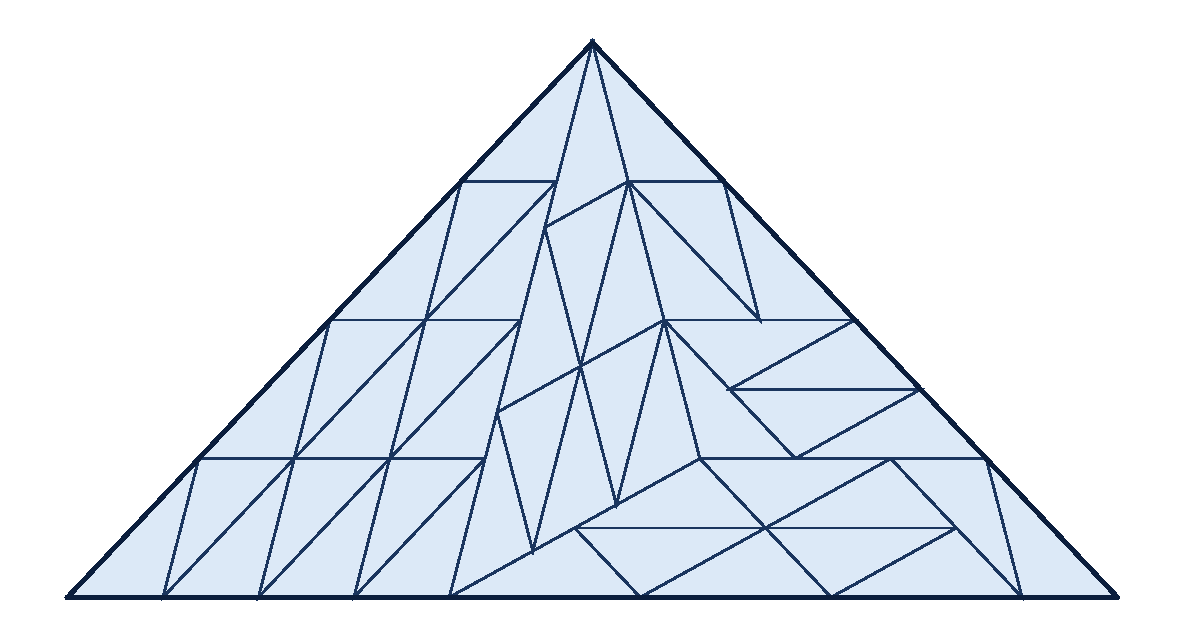
\includegraphics[width=0.72\linewidth]{tiling44.pdf}
\caption{The $44$-tiling of $(16,16,22)$ by the tile $(2,3,4)$, found by exhaustive search and
verified exactly. To our knowledge the first tiling in any of the three isosceles
$3\alpha+2\beta=\pi$ cases, and the smallest known triangle tiling in any incommensurable
branch (the previously smallest was Herdt's $1215$).}
\label{fig:44}
\end{figure}

Three remarks. First, $44$ is not a square, not a sum of two squares ($11\equiv3\bmod4$), and
not $2,3,6$ times a square: it is the first tile count \emph{outside the commensurable families}
to be certified realizable at small size, and the first new member of the tile-count set
discovered by these methods --- every other frontier value was excluded. Second, Beeson's
constructions in \cite{BeesonIII} cover the two scalene $3\alpha+2\beta=\pi$ shapes (his
triquadratic tilings, smallest $N=28$ --- which, we note, settles $28$'s membership and is used
in our accounting below); the isosceles cases had, to our knowledge, no known tiling, and the
smallest known tiling in any incommensurable branch was Herdt's $1215$. Third, the value
demonstrates that the small members of the $3\alpha+2\beta=\pi$ tables are not uniformly
impossible: each must be searched, and Theorem~\ref{thm:decidable}'s per-instance decision is
genuinely two-sided.

\subsection*{The values $51$, $55$, $57$, $62$, and the $\gamma=2\alpha$ boundary algorithm.}
The sweep continues past the forties. The values $51=3\cdot17$, $55=5\cdot11$ and $57=3\cdot19$
are squarefree, so the $\gamma=2\alpha$ branch is closed by \cite[Thm.~11.7]{BeesonIso}, and every
branch except isosceles-$(\alpha{+}\beta)$ dies arithmetically; each surviving instance is uniquely
determined and the engine exhausts all six ($62$ dies in every branch outright, as $42$ did):
\begin{center}
\begin{tabular}{llll}
instance & tile & target & nodes\\
\hline
$N{=}51$, $M{=}1$ & $(650,51,676)$ & $(1326,1326,1275)$ & $3649$\\
$N{=}51$, $M{=}3$ & $(70,51,100)$ & $(510,510,357)$ & $180$\\
$N{=}55$, $M{=}1$ & $(756,55,784)$ & $(1540,1540,1485)$ & $5911$\\
$N{=}55$, $M{=}5$ & $(24,55,64)$ & $(440,440,165)$ & $40$\\
$N{=}57$, $M{=}1$ & $(812,57,841)$ & $(1653,1653,1596)$ & $8961$\\
$N{=}57$, $M{=}3$ & $(88,57,121)$ & $(627,627,456)$ & $193$\\
$N{=}63$, $M{=}1$ & $(992,63,1024)$ & $(2016,2016,1953)$ & $15493$\\
$N{=}63$, $M{=}3$ & $(12,7,16)$ & $(84,84,63)$ & $44859$\\
$N{=}63$, $M{=}7$ & $(8,63,64)$ & $(504,504,63)$ & $2$\\
$N{=}69$, $M{=}1$ & $(1190,69,1225)$ & $(2415,2415,2346)$ & $37995$\\
$N{=}69$, $M{=}3$ & $(130,69,169)$ & $(897,897,690)$ & $523$\\
\end{tabular}
\end{center}
The three $N{=}63$ rows close its isosceles-$(\alpha{+}\beta)$ branch, and its $\gamma=2\alpha$
instance --- the boundary algorithm (below) leaves exactly one candidate, tile $(9,7,12)$ with
target $(63,63,84)$ --- is exhausted too, at $884921$ nodes, to our knowledge the first instance
decided \emph{inside} Beeson's ``swath of ignorance'' $[45,1125]$ for the $\gamma=2\alpha$ branch
\cite[\S11.6]{BeesonIso}. The value $63$ itself is nevertheless \emph{realizable}, through a
branch the sweep had marked as arithmetically dead: Theorem~\ref{thm:63} and
Remark~\ref{rem:63correction} below. The values $70$
and $78$ die in every branch outright, as $42$ and $62$ did. The value $66$ reduces to its
$\pi/3$-equilateral instance (tile $(11,96,91)$, side $264$, coloring number $M=4$), which Beeson
rejects \cite[Thm.~7]{BeesonEq}: the tiling must witness a relation $91j=11\ell+96m$ with
$91j<264$, and neither $j=1$ nor $j=2$ admits one. And $77$ goes the \emph{other} way: its
$(2\alpha,\alpha,2\beta)$ instance satisfies Beeson's second tiling equation at
$(M,s)=(5,\tfrac12)$ --- $25\cdot\frac{(2-\frac14)(3-\frac14)}{(1-\frac12)^2(2+\frac12)^2}=77$ ---
and his four-component construction \cite{BeesonIII} realizes every solution, so \emph{a triangle
can be cut into $77$ congruent triangles}: the $(2\alpha,\alpha,2\beta)$ triangle over the same
tile $(2,3,4)$ that Theorem~\ref{thm:44} uses for $44$. We need not rely on that construction: the
engine finds the tiling directly (node $849\,624$), and its certificate is \emph{machine-verified in
Lean~4 with no axioms whatsoever} (\texttt{lean/Tiling77.lean}: all $77$ triangles congruent to
$16\cdot(2,3,4)$ over $\Z[\sqrt{15}]$, contained in the target $16\cdot(28,16,33)$, an explicit
separating edge-line for each of the $2926$ pairs, and the exact area sum). The realizability of
$77$ therefore rests on a kernel-checked object rather than on a cited construction.

For values that are \emph{not} squarefree the $\gamma=2\alpha$ branch needs more than
Theorem~11.7. Beeson's isosceles paper provides exactly the needed machinery: the tile must be
$(k^2,\,m^2{-}k^2,\,mk)$ with $\gcd(k,m)=1$, $2k>m>k$ \cite[Lem.~11.2]{BeesonIso}; $m$ is bounded
in terms of $N$ \cite[Lem.~11.12]{BeesonIso}; the side $X$ and base $Y$ satisfy $X^2=Nab$,
$Y=(m/k)X$ and must decompose as $X=pa+qb+rc$ with $q,r\ge1$ and $p+q+r<(N{+}1)/4$
\cite[Lems.~11.11, 11.13]{BeesonIso} and $Y=ua+vb+wc$ with $v,w\ge1$ (the base version of
Lemma~11.13, whose pigeonhole proof is stated for the base); and the pair is rejected when every
$X$-representation has $r=1$ while every $Y$-representation has $w\in\{1,2\}$
\cite[Lem.~11.17]{BeesonIso}. We implemented this boundary algorithm independently
(\texttt{code/gamma2alpha.py}) and calibrated it against Beeson's reported results: it excludes
$20$, $28$ and $44$ and leaves $45$ surviving via the tile $(4,5,6)$, exactly as in
\cite[Thm.~11.18]{BeesonIso}; at $36$ our filter is strictly weaker than Beeson's direct argument
(it reports a surviving boundary representation), so we use it only in the sound direction.
Running it on the undetermined values: \emph{the $\gamma=2\alpha$ branches at $N=56$ and $N=60$
are empty} --- no possible boundary tiling exists.

Consequently $N=56$ reduces far: $\gamma=2\alpha$ is closed by the algorithm, both
isosceles-$(\alpha{+}\beta)$ instances are exhausted by the engine ($M{=}2$: tile $(195,56,225)$,
target $(840,840,728)$, $853$ nodes; $M{=}4$: tile $(45,56,81)$, target $(504,504,280)$, $89$
nodes), and every other branch dies arithmetically --- \emph{except} the $2\pi/3$-equilateral
instance: tile $(8,7,13)$, equilateral target of side $56$, from the factorization
$(s,t)=(12,14)$ of Proposition~\ref{prop:eqspec}. The membership of $56$ is thus equivalent to
that single equilateral instance --- and the engine \emph{exhausts it}: no tiling exists, at
$156646$ nodes, identically in both independent engine implementations (node-for-node
agreement). Likewise $N=60$ reduces to its equilateral instance alone (tile $(5,3,7)$, side
$30$): its two isosceles-$(\alpha{+}\beta)$ instances are exhausted as well ($M{=}2$: tile
$(56,15,64)$, target $(240,240,210)$, $123003$ nodes; $M{=}6$: tile $(4,15,16)$, target
$(120,120,30)$, $39$ nodes) --- and the equilateral instance itself is exhausted at $853731$
nodes: $N=60$ is excluded. (This also settles the $m{=}2$ member $X=30$ of Zhang's
equiconstructibility family for $(5,3,7)$ by exact arithmetic; Beeson had reported $X<105$
unrealizable for this tile in unpublished floating-point work.)

\begin{theorem}\label{thm:frontier3}
No triangle can be cut into $51$, $55$, $56$, $57$, $60$, $62$, $69$, or $78$
congruent triangles.
\end{theorem}

\begin{proof}
The branch sweeps and the exhaustive searches above; dependencies as in
Theorem~\ref{thm:frontier}, together with \cite[Thm.~11.7]{BeesonIso} for the $\gamma=2\alpha$
branch at the squarefree values $51$, $55$, $57$, $69$; the boundary algorithm (Lemmas 11.2--11.17 of
\cite{BeesonIso}, \texttt{code/gamma2alpha.py}) for the $\gamma=2\alpha$ branch at $56$ and
$60$; and the $7\,232\,464$-node exhaustion at $66$ (Remark~\ref{rem:isobeta}).
\end{proof}

\begin{theorem}[$63$ is realizable]\label{thm:63}
A triangle can be cut into $63$ congruent triangles: the scalene triangle with sides $(21,24,18)$
--- angles $(\beta,\,2\alpha,\,\alpha{+}\beta)$ over the same tile $(2,3,4)$ as
Theorem~\ref{thm:44} --- is tiled by $63$ congruent copies of that tile. The tiling is exhibited
exactly and its certificate is machine-verified in Lean~4 with no axioms
(\texttt{lean/CevianTiling63.lean}: all $63$ triangles congruent to $8\cdot(2,3,4)$ over
$\Z[\sqrt{15}]$, contained in the closed target $8\cdot(21,24,18)$ by half-plane checks, an
explicit separating edge-line for each of the $1953$ pairs, and the exact area identity), and it
was re-verified independently of the kernel by a second exact sweep with the separating axes
recomputed from scratch (\texttt{code/interface\_census.py}). Consequently $63m^2$ is a tile
count for every $m\ge1$. The same shape at count $28$ is \texttt{lean/CevianTiling28.lean}; the
two are the $m=3$ and $m=2$ members of the cevian family $N=m^2(2f^2-e^2)$ at $(e,f)=(1,2)$
(companion note, realizability section).
\end{theorem}

\begin{remark}[Correction, and its scope]\label{rem:63correction}
An earlier version of this paper listed $63$ among the excluded values of
Theorem~\ref{thm:frontier3}. That was wrong: the branch sweep treated the scalene
$3\alpha+2\beta=\pi$ shapes as arithmetically dead at $63$, and Theorem~\ref{thm:63} refutes that
step by certificate. The per-instance exhaustions quoted in these subsections are unaffected ---
each is a statement about a single (tile, target) pair and stands --- but every \emph{composite}
exclusion below $90$ also invokes the sweep's claim that the branches absent from its surviving
lists die arithmetically, and that claim has now produced one false exclusion. The re-audit of
the sweep is complete, and the error is a single filter: the scalene step found the
representation $N=2K^2-M^2$ and then applied the divisibility $K\mid M^2$ recorded from
\cite[Thm.~7]{BeesonIII}. Writing $g=\gcd(M,K)$ and $(e,f,m)=(M/g,K/g,g)$, the representation is
exactly the cevian family $N=m^2(2f^2-e^2)$ and the filter reads $f\mid m$ --- refuted outright
by the certificate of Theorem~\ref{thm:63} ($m=3$, $f=2$; the value $28$ passed only because
$f\mid m$ happens to hold there, which is why the error stayed invisible until $63$). The filter
is the same unsound divisibility class as \cite[Thms.~14, 19]{BeesonIII}
(Remark~\ref{rem:b3prime}), whose analogues the sweep already declines to apply. With the filter
removed the sweep was re-run over every composite exclusion below $90$
(\texttt{verify\_frontier.py}, with a self-test pinning the corrected branch on the certified
members $63$ and $28$): exactly four values acquire a live scalene instance, all cevian ---
$N=14$ at $(e,f,m)=(2,3,1)$, tile $(6,5,9)$ on $(15,28,27)$; $N=46$ at $(2,5,1)$, $(10,21,25)$ on
$(105,92,125)$; $N=56$ at $(2,3,2)$, $(6,5,9)$ on $(30,56,54)$; and $N=62$ at $(6,7,1)$,
$(42,13,49)$ on $(91,372,343)$ --- and every other composite exclusion below $90$ is confirmed:
its scalene branch is empty, and its surviving instances are the ones already settled by the
quoted per-instance exhaustions. All four reopened instances are excluded by exhaustive search
(verified: $14$ at $678$ nodes, $46$ at $4\,685$, $56$ at $4\,890\,763$, $62$ at
$12\,872\,188$; instances generated by \texttt{code/engine/gen\_cevian.py}, byte-exact against
the certified members). The re-audit is therefore closed: every composite exclusion below $90$
stands, now with the corrected sweep and the four cevian exhaustions in its dependency list, and
the sole change to the paper's conclusions remains the realizability of $63$ itself
(Theorem~\ref{thm:63}). The prime exclusions are untouched throughout, resting on
Theorem~\ref{thm:main} and the congruence class alone.
\end{remark}

\begin{corollary}[The cevian spectrum at $(1,2)$ is complete]\label{cor:wfamily}
The scalene target of Theorem~\ref{thm:63} realizes $N=7m^2$ for every $m\ge2$ and for no other
$m$: the certified seeds $W_2=28$ and $W_3=63$ propagate by the W-addition law of the companion
note (the connecting parallelograms are slab-tiled by the $c$-glued two-tile brick), every
$m\ge2$ being a sum of $2$s and $3$s; and a $7$-tiling at $m=1$ would extend, by the east
$f$-scaled tile, to an $11$-tiling of $(8,8,11)$, refuted by exhaustion. This is a second
(target, tile) pair with no undecided instance, over the same tile $(2,3,4)$ as
Theorem~\ref{thm:realize12}; it adds $175=7\cdot5^2$ to the spectrum below $200$.
\end{corollary}

\begin{remark}[The value $70$ and the unsound $g\mid M$ exclusions]\label{rem:seventy}
The value $N=70$ is excluded. Its single surviving instance is isosceles-$\alpha$: tile $(6,5,9)$,
$M=8$, target $(45,45,70)$, which passes the tiling equation \emph{and} side-integrality ($X=45$,
and indeed $(2f+e)=8\mid M$); the previously published exclusion rested solely on $g\mid M$ from
\cite[Thm.~19]{BeesonIII} ($g=3\nmid8$), whose proof is unsound (Remark~\ref{rem:b3prime}), and
Beeson's own Table~5 marks this very instance ``?''. The exhaustive search settles it directly:
the instance admits no tiling ($134\,631\,158$ nodes, walk- and corner-pruned). The exclusion of
$70$ therefore rests on the search rather than on \cite[Thm.~19]{BeesonIII}. The value
$21$, whose analogous isosceles-$\alpha$ candidate (tile $(2,3,4)$, $M=5$,
target $(12,12,21)$) was likewise previously killed only by the unsound $g\mid M$, \emph{is}
excluded: the engine exhausts the instance ($13\,659$ nodes, no tiling), so
Theorem~\ref{thm:frontier2} stands with its dependence on \cite[Thm.~19]{BeesonIII} removed. The
same applies to $N=39$, whose base-$\beta$ candidate (tile $(12,7,16)$ on $(64,64,117)$) the engine
exhausts in $825\,724$ nodes: Theorem~\ref{thm:frontier2} therefore stands for $39$ as well,
independently of \cite[Thm.~14]{BeesonIII}. Of the values whose exclusion rested on an unsound
divisibility, only $70$ remains pending (Remark~\ref{rem:seventy}); $59$ and $66$ have since been
exhausted by exact search, at $1\,838\,175$ and $7\,232\,464$ nodes respectively.
\end{remark}

\begin{remark}
The $2\pi/3$-equilateral exhaustions at $N=56$ (tile $(8,7,13)$, side $56$) and $N=60$ (tile
$(5,3,7)$, side $30$) lie strictly inside the range $12<N<1215$ that Beeson leaves \emph{open} for
this case --- he proves only $N\ge12$ \cite[\S5]{BeesonEq} --- and, cross-checked to the node in
two independent engine implementations ($156\,646$ and $853\,731$ nodes respectively), are to our
knowledge the first rigorous exclusions inside it. The value $56$ moreover settles the $m{=}1$ case
of Zhang's equiconstructibility family for $(8,7,13)$: the side-$56$ equilateral is \emph{not}
tileable by $(8,7,13)$, exactly as Zhang's Conjecture~2 predicts (his construction realizes $X=56m$
only for $m\ge9$). It also closes the $m{=}1$ route of his Proposition~9(1) to the $F_1$ instance
$N=105$: any $105$-tiling of $(105,56,91)$, if one exists, does not factor through an equilateral
$56$-block.
\end{remark}

\subsection*{The values $76$ to $80$.}
The same branch sweep (\texttt{verify\_frontier.py}) extends the determined initial segment past
$75$. For $N=76=4\cdot19$ the only live branches are $\gamma=2\alpha$ (excluded by the boundary
algorithm of Lemmas 11.2--11.17 of \cite{BeesonIso}, \texttt{code/gamma2alpha.py}) and the
$3\alpha+2\beta=\pi$ isosceles-$(\alpha{+}\beta)$ target with tile $(90,19,100)$ on the isosceles
$(380,380,342)$, which the engine exhausts ($955\,474$ nodes); every other branch is dead by its
$N$-form. Hence $76$ is not realizable. The prime $79\equiv3\pmod4$ is excluded by
Theorem~\ref{thm:main}; and $77$, $80$ are realizable --- $77$ by Beeson's four-component
construction \cite{BeesonIII}, and $80=4^2+8^2$ by the biquadratic (commensurable) tiling
\cite{BeesonSeven}.

\begin{theorem}\label{thm:frontier4}
No triangle can be cut into $76$ congruent triangles. Every $N\le 80$ is thereby determined,
with no exception: the realizable values are exactly $1$--$13$'s known members together with
$44,63,77,80$ and the standard commensurable and prime\,$\equiv1\!\pmod4$ values, and all others
are excluded. The last undetermined value below $80$ was $N=70$, settled by exhaustive search of
its single surviving instance (Remark~\ref{rem:seventy}).
\end{theorem}
\begin{proof}
The branch sweep and $\gamma=2\alpha$ boundary algorithm above settle $76$; Theorem~\ref{thm:main}
excludes the prime $79$; Theorems~\ref{thm:frontier2}--\ref{thm:frontier3} give the composite
exclusions through $78$ other than $70$; and Theorem~\ref{thm:63}, the four-component and
biquadratic constructions realize $63$, $77$ and $80$.
\end{proof}

\subsection*{The values $81$ to $90$.}
The sweep continues past $80$ with no change of method. Five values are realizable outright by the
commensurable construction, being sums of two squares: $81=9^2$, $82=1^2+9^2$, $85=2^2+9^2$,
$89=5^2+8^2$, $90=3^2+9^2$. The prime $83\equiv11\pmod{12}$ is excluded by
Theorem~\ref{thm:fullprime}. For $86$ every branch is dead by its $N$-form. That leaves $84$, $87$
and $88$, at which the $\gamma=2\alpha$ branch is alive by $N$-form ($84$ and $88$ are not
squarefree) and is killed by the boundary algorithm of Lemmas 11.2--11.17 of \cite{BeesonIso}
(\texttt{code/gamma2alpha.py}: $82$--$89$ all return \emph{no possible boundary tiling}; the
survivors in the band are $81$ and $90$, both already realizable). The surviving instances are then
finitely many isosceles $3\alpha+2\beta=\pi$ targets with a uniquely determined tile, and the engine
decides each:
\[
\begin{array}{llll}
N=87: & (208,87,256) \text{ on } (1392,1392,1131), & 2\,107 \text{ nodes}; \\
      & (1892,87,1936) \text{ on } (3828,3828,3741), & 278\,197 \text{ nodes};\\
N=88: & (117,88,169) \text{ on } (1144,1144,792), & 489 \text{ nodes}; \\
      & (483,88,529) \text{ on } (2024,2024,1848), & 15\,493 \text{ nodes}.
\end{array}
\]
All four are exhausted with no tiling. For $87$ that settles the value. For $88$ one further
instance must be treated, from a family that cannot arise below it; see
Remark~\ref{rem:F4at88}.

\begin{theorem}\label{thm:frontier5}
No triangle can be cut into $86$ or $87$ congruent triangles. In the range $81\le N\le 90$ the
realizable values are exactly $81,82,85,89,90$; $86$ and $87$ are excluded unconditionally; $83$ is
excluded under the hypothesis of Theorem~\ref{thm:fullprime} and not otherwise
(Remark~\ref{rem:eightythree}); and $84$ and $88$ remain open, each awaiting the exhaustion of
instances currently under search.
\end{theorem}
\begin{proof}
For $86$ every branch is dead by its $N$-form (commensurable, tile-similar, right-angle and the four
$3\alpha+2\beta=\pi$ shapes all fail their defining equations; the $2\pi/3$ spectra of
Theorems~\ref{thm:frontier2}--\ref{thm:frontier3} exclude it, and the scalene $2\pi/3$ shapes cannot
reach it by Remark~\ref{rem:F4at88}; $\gamma=2\alpha$ dies because $86$ is squarefree). For $87$ the
same sweep leaves the two instances tabulated above, each exhausted by the exact search of
Section~\ref{sec:verification}. The realizable values are sums of two squares as listed, and $83$ is
Theorem~\ref{thm:fullprime}.
\end{proof}

\begin{remark}[The scalene $2\pi/3$ shape $F_4$ first becomes possible at exactly $88$]\label{rem:F4at88}
Recorded in \cite{Obstructions}.
\end{remark}

\begin{remark}[The third isosceles base-$\alpha$ instance]\label{rem:isoalpha84}
Recorded in \cite{Obstructions}.
\end{remark}

\begin{remark}[What $83$ rests on]\label{rem:eightythree}
Recorded in \cite{Obstructions}.
\end{remark}

\subsection*{The spectrum below $200$.}
The determinations above assemble into an explicit answer to Erd\H{o}s's question on the initial
segment $N\le200$ (generated by \texttt{code/spectrum\_table.py}; every entry cites its reason).
The \emph{realizable} values, $100$ of the $200$, are the unions of six families: the squares
$k^2$; the sums of two positive squares $x^2+y^2$ (the biquadratic right-triangle tiling, covering
$2$ and every prime $\equiv1\bmod4$); $3k^2$ and $6k^2$ (equilateral trisection and sextant);
the certified incommensurable values $28$, $44$, $63$, $77$, $99$ of this paper and its companion;
the cevian family $7m^2$, $m\ge2$ (companion, W-addition), whose first member beyond the
certified ones is $175=7\cdot5^2$; and the $k^2$-ladder over all of these
(Theorem~\ref{thm:ladder}), which contributes $112=2^2\cdot28$ and $176=2^2\cdot44$. Explicitly:
\[
\begin{array}{l}
1,2,3,4,5,6,8,9,10,12,13,16,17,18,20,24,25,26,27,28,29,32,34,36,37,40,41,44,45,48,49,50,\\
52,53,54,58,61,63,64,65,68,72,73,74,75,77,80,81,82,85,89,90,96,97,98,99,100,101,104,106,\\
108,109,112,113,116,117,121,122,125,128,130,136,137,144,145,146,147,148,149,150,153,157,\\
160,162,164,169,170,173,175,176,178,180,181,185,192,193,194,196,197,200.
\end{array}
\]
The \emph{excluded} values, $42$ in number, are the primes $\equiv7\bmod{12}$
($7,19,31,43,67,79,103,127,139,151,163,199$; Theorem~\ref{thm:main} with
Theorem~\ref{thm:mod12}, unconditional), the exhausted primes $\equiv11\bmod{12}$
($11,23,47,59,71,107$), and the composite values of
Theorems~\ref{thm:frontier}--\ref{thm:frontier5}
($14,15,21,22,30,33,35,38,39,42,46,51,55,56,57,60,62,66,69,70,76,78,86,87$), the last group
subject to the branch-sweep caveat of Remark~\ref{rem:63correction} until the scalene re-audit
closes. Everything else is \emph{open}, $58$ values:
\[
\begin{array}{l}
83^{*},84,88,91,92,93,94,95,102,105,110,111,114,115,118,119,120,123,124,126,129,131^{*},132,\\
133,134,135,138,140,141,142,143,152,154,155,156,158,159,161,165,166,167^{*},168,171,172,174,\\
177,179^{*},182,183,184,186,187,188,189,190,191^{*},195,198,
\end{array}
\]
where the starred values are the unresolved primes $\equiv11\bmod{12}$ ($83$ is excluded under
the base-$\beta$ hypothesis and not otherwise, Theorem~\ref{thm:frontier5}); $84$ and $88$ are
the two instances still under search below $91$; $105,120,132,154,184$ are the sporadic
$2\pi/3$-admissible values of Remark~\ref{rem:zhang}; and $66$'s and $138$'s base-$\beta$ members
are exhausted while the values themselves differ in kind --- $66$ is excluded
(Theorem~\ref{thm:frontier3}), $138$ merely branch-dead in base-$\beta$ and otherwise open.
Below $91$ the spectrum is thus determined except at exactly $83$, $84$, $88$; the first open
composite is $84$.

\subsection*{Decidability.}
The pattern of the last two subsections is not an accident. Every branch of the classification now
reduces, for each fixed $N$, to a \emph{finite} list of fully determined instances: the
commensurable, similar-tile, right-angle and $\gamma=2\alpha$ branches are decided by closed
$N$-forms; in the sporadic $2\pi/3$ shapes the divisor structure of $N$ (Theorems
\ref{thm:admissible}, \ref{thm:lattice}, Proposition~\ref{prop:otherspectra}) leaves finitely
many (tile, scale) pairs; the equilateral cases pin the tile from finitely many factorizations
(Proposition~\ref{prop:eqspec}) or coloring numbers (\cite[Thm.~2]{BeesonEq}, which determines
the tile from $(N,M)$); and the five $3\alpha+2\beta=\pi$ shapes have finitely many $(M,s)$
candidates by their tiling equations~\cite{BeesonIII}. Each surviving instance is a bounded
existence question, and the corner-anchored search of \texttt{code/engine/} decides it in
finitely many steps (the branching is provably complete and the depth is $N$). Hence:

\begin{theorem}[Decidability]\label{thm:decidable}
It is decidable, given $N$, whether some triangle can be cut into $N$ congruent triangles
(under the same cited inputs as Theorem~\ref{thm:main}).
\end{theorem}

\noindent This extends the decidability that Beeson established for equilateral
targets~\cite[Thm.~4]{BeesonEq} to the whole problem. What decidability does \emph{not} give is
a closed-form description of the set. After Theorem~\ref{thm:spectrum} and
Proposition~\ref{prop:conic}, the necessary side is closed in \emph{every} branch --- the
admissible values are Zhang's families in the sporadic shapes and explicit divisor-instances in
the equilateral cases --- so the entire residual openness of the problem is a single question:
\emph{which admissible instances are realized}. Zhang's trapezoid constructions realize the
sporadic families for $m\ge9$ in residue classes, and Laczkovich's elliptic-curve
analysis~\cite{LaczkovichEll} governs equilateral realizability; the open kernel is the small
members that are not already realized commensurably --- sharpest $N=105$ on the $F_1$ target of
$(8,7,13)$ --- and each such instance is individually decidable (Theorem~\ref{thm:decidable}).

\begin{remark}[no invariant decides realizability]\label{rem:conserved}
No invariant of the conserved type decides realizability. Full discussion in \cite{Obstructions}.
\end{remark}

\begin{remark}[the tiling group collapses as well]\label{rem:tilinggroup}
Recorded in \cite{Obstructions}.
\end{remark}

\subsection*{State of the full problem.}
Assembling: the commensurable branch is completely determined (squares, sums of two squares, and
$2,3,6$ times squares, all realized \cite{BeesonSeven}); the similar-tile and right-angle branches
are settled in \cite{BeesonI, SWW}; the primes are settled by Theorem~\ref{thm:primefull}. What
remains open for the full determination of the tile-count set is: sufficiency in the sporadic
$2\pi/3$ branches (Zhang's completeness conjecture~\cite{Zhang}; the admissible spectra above are
the outer bounds), the $3\alpha+2\beta=\pi$ and $\gamma=2\alpha$ branches beyond the partial
results of \cite{BeesonIII, BeesonIso}, and the equilateral targets for incommensurable tiles,
where Laczkovich has connected the possible $N$ to rational points on elliptic
curves~\cite{LaczkovichEll}. With $7$ and $11$ excluded by \cite{BeesonSeven}, the primes by Theorem~\ref{thm:primefull},
$14,15,21,22,30,33,35,38,39,42,46$ by Theorems \ref{thm:frontier} and~\ref{thm:frontier2},
$51,55,56,57,60,62,63,66,69,78$ by Theorem~\ref{thm:frontier3} ($70$ pending,
Remark~\ref{rem:seventy}), \emph{$44$ realizable} by
Theorem~\ref{thm:44}, $77$ realized by Beeson's four-component construction \cite{BeesonIII},
$28$ realized by his triquadratic tilings \cite{BeesonIII}, and the remaining values
commensurably realized ($45,48,49,50,52,53,54,58,61,64,65,68,72,73,74,75$) or prime
($47,53,59,67,71$), the membership of \emph{every $N\le75$} is now determined. The value $N=76$ is
likewise excluded ($\gamma=2\alpha$ empty by the boundary algorithm; its one
isosceles-$(\alpha{+}\beta)$ instance, tile $(90,19,100)$ on $(380,380,342)$, exhausted by the
engine at $955\,474$ nodes); with $79$ prime (Theorem~\ref{thm:main}) and $80=4^2+8^2$ realized,
\emph{every $N\le80$ except the pending $70$} is now determined (Theorem~\ref{thm:frontier4}).

\subsection*{Progress on the base-$\beta$ branch.}\label{sub:basebetaprogress}
Theorem~\ref{thm:fullprime} is conditional on Hypothesis (walls) for the branch
$3\alpha+2\beta=\pi$ at $m=1$. The companion records the following unconditional
progress on that hypothesis, and also an unresolved tension between its corner-block statement and the
reading of it as ``no $a$-edge on an equal side'' that the side arguments use.

Before turning to the hypothesis we record an arithmetic fact that fixes, once and for all, which
prime candidates the two halves of Theorem~\ref{thm:fullprime} can reach. It is proved by an exact
identity rather than by any modular inversion, and it converts what had been a census into a
statement about all primes.

\begin{proposition}[Uniqueness of the base-$\beta$ representation]\label{prop:repunique}
Let $p$ be a prime and suppose $p=3f_1^2-e_1^2=3f_2^2-e_2^2$ with $1\le e_i<f_i$ and
$\gcd(e_i,f_i)=1$ for $i=1,2$. Then $(e_1,f_1)=(e_2,f_2)$. Consequently a prime candidate lies in
the $e=1$ family if and only if it has the form $3f^2-1$, and no prime of that form admits any
representation with $e\ge2$.
\end{proposition}

\begin{proof}
Eliminating $p$ between the two equations gives the exact identity
\[
  (e_1f_2)^2-(e_2f_1)^2 \;=\; p\,(f_1^2-f_2^2),
\]
obtained as $-f_2^2$ times the first equation plus $f_1^2$ times the second. Hence $p$ divides the
product $(e_1f_2-e_2f_1)(e_1f_2+e_2f_1)$. Admissibility bounds the parameters: from $e<f$ we get
$p=3f^2-e^2>2f^2$, so $2f_i^2<p$ for both $i$, and therefore $2f_1f_2<p$ by the arithmetic--geometric
inequality. Since $e_i<f_i$, both $e_1f_2$ and $e_2f_1$ are strictly less than $f_1f_2<p/2$, and both
are positive. Their \emph{sum} therefore lies strictly between $0$ and $p$ and cannot be divisible by
$p$; so $p$ divides the \emph{difference}, which lies strictly between $-p$ and $p$ and is hence $0$.
Thus $e_1f_2=e_2f_1$. Coprimality of each pair gives $e_1\mid e_2$ and $e_2\mid e_1$, so $e_1=e_2$,
and cancelling the nonzero $e_1$ yields $f_1=f_2$.
\end{proof}

The proposition is formalised as \texttt{Erdos634.ThinHole.rep\_unique}, axiom-clean. It explains the
census that motivated it: the primes representable only at $e=1$ --- $11,47,107,191,431,587,971,\dots$,
$82$ of them below $600\,000$ --- are exactly the primes of the form $3f^2-1$, and this is now a
theorem rather than an observation. In particular the unconditional $e\ge2$ half of
Theorem~\ref{thm:fullprime} is not merely unhelpful on these candidates: it is \emph{provably}
inapplicable to them, so the $e=1$ argument is not redundant with it on any prime.

For the thin subfamily $e=1$ the hypothesis holds for $f\le6$, that is for the members with
$N=3f^2-1$ equal to $11,26,47,74,107$. For two of them the corresponding $m=1$ target is in
addition shown to admit no tiling by an independent exhaustive search ($132\,519$ nodes at
$f=5$ and $1\,251\,382$ at $f=6$). These searches concern one instance each and are statements
about the base-$\beta$ branch at $m=1$; they are not exclusions of the integers themselves, and
indeed $74=5^2+7^2$ is a tile count by the commensurable construction.

For $e\ge2$ the base walk is now determined. The walk of a separated member, meaning one with
$f^2>2ef+e^2$, admits exactly three edge decompositions; the $\gamma$-trap deletes the one with no
$c$-edge, and the remaining non-walls column $(0,e,2e)$ is excluded outright: with no $a$-edge on
the base each corner tile lays $c$ on the base and $a$ on the side, the unique fills of $\beta$,
$\alpha$ and $\alpha+\beta$ force the corner partner and then every subsequent one, and the base is
driven to consist of $c$-edges alone, which would require $f^2\mid e^3$. Hence at a separated
thick member the base walk is the walls form, with $f$ $a$-edges, $e$ $b$-edges and $e$ $c$-edges.
For three thick members the $m=1$ target is likewise exhausted, establishing the hypothesis
there: $(e,f)=(2,3)$, $(2,5)$ and $(3,4)$, with $N=23$, $71$ and $39$ and node counts
$19\,677$, $553\,417$ and $825\,724$. The first two of these integers are primes congruent to
$11$ modulo $12$; all three are already excluded as tile counts by other means recorded above.

A further reduction of the side condition is now available. The apex of a base-$\beta$ target is
rigid, and the rigidity is an identity of the whole family: $b\cos\frac{\alpha}{2}=c\cos\frac{3\alpha}{2}$
for every $(e,f)$, which places the apex tile's third vertex exactly on the chord through the first
junction of an equal side, so that its $a$-edge lies \emph{along} that chord and has length exactly
$a$. The area above that chord is $2+b/c=N/f^{2}$ tile areas, filled by the two outer apex tiles
together with the fraction $b/c$ of the middle one and by nothing else, so that chord is met from
above by exactly three tiles. It follows that the edge of an equal side immediately below the first junction is again a $c$, whence
$n_c\ge2$ and
\[
pe+2\le f .
\]
This holds at every member with $\gcd(e,f)=1$. The step needs only that the tile below cannot lay a
$b$-edge towards the junction, and when $b<a$ that is forced by a semigroup argument: the residual
length $a-b$ satisfies $a-b\equiv-f^{2}\pmod e$, so any representation over $\langle a,b,c\rangle$
would need at least $e-1$ copies of $b$ or $c$, giving $a-b\ge(e-1)b$, whereas $(e-1)b>a-b$ because
$b>f$ holds at every member.
In particular $p=2$ is excluded on the whole tight subfamily $f=2e+1$, by an argument independent of
the chord and height estimates used there previously.

Removing the hypothesis has one further consequence, on the family $e=f-1$, which the earlier form
could not reach because $f/(f-1)$ lies below the golden ratio for every $f\ge3$. There
$n_c=f-p(f-1)$, which is $1$ at $p=1$ and non-positive for $p\ge2$; both contradict the bound. Hence
$p=0$ on every equal side at \emph{every member with $e=f-1$}: no equal side carries an $a$-edge, which is
Hypothesis (walls) at those members under the reading discussed in the companion. The tile counts are $N=2f^{2}+2f-1$, and the base-$\beta$ candidates among them --- primes
congruent to $11$ modulo $12$ --- beyond the range already determined are
$83$, $179$, $263$, $311$, $419$, $479$, $683$, $839$, $1103$, $1511$, $2111$, $2243$, $2663$, $2963$,
$3119$ for $f\le39$. This discharges the hypothesis at those members; it does not by itself settle the
integers, which needs the remaining branches. The argument is written out in the companion, where its
label is recorded as PROVED with the outstanding formalization and review noted. The bound does not reach $p=1$ at any new
member: that would need $e\ge f-1$, and $pe+2\le f$ then gives $f\le e+1\le pe+2-e+1$, leaving only
the smallest members, all already closed.

The residual question has correspondingly sharpened. Each junction $J$ of an equal side whose upper
edge is a $c$ determines a point $W(J)$ on the chord through $J$, at distance exactly $a$ from $J$,
namely the third vertex of the $c$-tile above. An $a$-edge immediately below $J$ forces $W(J)$ to lie
interior to an edge of some tile. Hence the hypothesis holds at any member with $e^{2}+ef<f^{2}$
provided no such $T$-junction occurs. At the first junction none does, because two tiles present
$\gamma$ there; at every later junction the configuration is a verbatim copy of the first, and a lone
$\gamma$ beside a straight edge is always consistent because $\alpha+\beta+\gamma=\pi$, so no counting
argument can settle it. All of this is proved in the companion and the identities are machine-checked
(\texttt{lean/ApexRigidity.lean}, \texttt{lean/SecondEdge.lean}).

On the tight subfamily $f=2e+1$ the standing hypothesis is automatic --- $e^{2}+ef<f^{2}$ there reduces
to $e^{2}+3e+1>0$ --- so $pe\le 2e-1$ and $p\le1$ at every member. The members of that subfamily whose
tile count $N=11e^{2}+12e+3$ is a prime congruent to $11$ modulo $12$ and is still open are
\[
\begin{array}{rrrl}
N & e & f & \text{tile }(a,b,c)\\\hline
227 & 4 & 9 & (36,65,81)\\
1223 & 10 & 21 & (210,341,441)\\
3011 & 16 & 33 & (528,833,1089)\\
4643 & 20 & 41 & (820,1281,1681)\\
5591 & 22 & 45 & (990,1541,2025)\\
8963 & 28 & 57 & (1596,2465,3249)\\
13127 & 34 & 69 & (2346,3605,4761)
\end{array}
\]
together with $N=138$ at $(3,7)$, which is not prime but is the smallest member where the question is
live. Each of the eight is in the same state: base walk settled, $p\in\{0,1\}$, and the single open
question $p=1$. No step of the argument uses the member beyond $e^{2}+ef<f^{2}$, so a proof at one is
a proof at all eight; an exhaustive search, by contrast, reaches only the member it is run on, the
next target after $N=138$ having a triangle nine times larger in linear scale.

What remains for the hypothesis in general is the side condition, namely the exclusion of
$1\le p\le(f-2)/e$ where $fp$ is the number of $a$-edges on a side, together with the members
with $f\le(1+\sqrt2)e$, for which the base walk admits further columns. Both reduce to one
question: whether the tile across a corner-chain $b$-edge lays a whole $b$ there. At the corner
itself that $b$-edge joins a base vertex to a side vertex and the answer is yes unconditionally;
one step in, its upper end is interior, and the configurations in which an edge overruns such an
end occur in genuine partial configurations at every scale examined, including $m=1$.
\subsection*{Standing of the inputs.}
The external inputs to Theorem~\ref{thm:main} and their publication status are as follows:
Laczkovich's classification papers \cite{Laczkovich1995,Laczkovich2012} and the rep-tiling theorem
of Snover--Waiveris--Williams \cite{SWW} are refereed journal articles, and Beeson's isosceles
paper \cite{BeesonIso} is accepted (to appear in \emph{Integers}); Beeson's remaining branch papers
\cite{BeesonI,BeesonIII,BeesonSeven,BeesonEq} and the Beeson--Zhang rationality
theorem~\cite{BeesonZhang}, which is load-bearing for the integrality of the tile, are arXiv
preprints at the time of writing. Zhang's constructions~\cite{Zhang} are cited for context only and
carry no logical weight here. The parts original to this paper (Sections
\ref{sec:reduction}--\ref{sec:isosceles} and \ref{sec:full}, together with the shape enumeration
of Section~\ref{sub:shapes}) are self-contained given those inputs, with the arithmetic layer
machine-checked (Section~\ref{sec:verification}).

\section{Verification}\label{sec:verification}

Every finite and numerical claim in this paper is checked in exact arithmetic by the scripts in the
repository, and the arithmetic and combinatorial layers are machine-checked in Lean~4 with Mathlib:
$144$ modules, $1491$ theorems, no \texttt{sorry}, and no axioms beyond the three Mathlib standard ones.
The four realizations used below --- the $28$-, $44$-, $77$- and $99$-tilings --- are certified by
kernel-checked certificates, each verifying that the pieces are congruent to the stated tile,
positively oriented, contained in the target, pairwise separated by explicit lines, and of total area
equal to the target's.

A statement-by-statement table, giving for each numbered claim the script or Lean declaration that
checks it and naming the claims that are \emph{not} formalized together with the reason, is in
\texttt{lean/PAPER\_MAP.md} in the repository; the searches, their instances and their node counts are
listed in \cite{Obstructions}.

\begin{thebibliography}{99}

\bibitem{Companion} V.~Bonfioli, \emph{The base-$\beta$ branch of $3\alpha+2\beta=\pi$: boundary walks, corrections to Triangle Tiling III, and the frontier searches}, companion note to the present paper, 2026.

\bibitem{Obstructions} V.~Bonfioli, \emph{Erd\H{o}s Problem 634: obstructions, scope limits, and closed routes}, 2026.

\bibitem{BeesonI} M.~Beeson, \emph{Triangle tiling I: The tile is similar to ABC or has a right
angle}, arXiv:1206.2231.

\bibitem{BeesonNoPrime} M.~Beeson, \emph{No prime tiling of an isosceles triangle},
  arXiv:2607.19572 [math.MG], 21 July 2026.

\bibitem{BeesonIII} M.~Beeson, \emph{Triangle tiling III: the case $3\alpha+2\beta=\pi$},
arXiv:1206.2229.

\bibitem{BeesonIso} M.~Beeson, \emph{Tilings of an isosceles triangle}, arXiv:1206.1974; to appear
in Integers.

\bibitem{BeesonSeven} M.~Beeson, \emph{No triangle can be cut into seven congruent triangles},
arXiv:1811.09723.

\bibitem{BeesonEq} M.~Beeson, \emph{Tiling an equilateral triangle}, arXiv:1812.07014.

\bibitem{BeesonZhang} M.~Beeson and Y.~X.~Zhang, \emph{Rationality of certain triangle tilings},
arXiv:2604.01314.

\bibitem{Zhang} Y.~X.~Zhang, \emph{Tiling triangles with $2\pi/3$ angles}, arXiv:2512.22696.

\bibitem{Erdos633} M.~Beeson, M.~Laczkovich and Y.~X.~Zhang, \emph{Solution of Erd\H{o}s
Problem~633}, arXiv:2604.03609.

\bibitem{Laczkovich1995} M.~Laczkovich, \emph{Tilings of triangles}, Discrete Math.\ \textbf{140}
(1995), 79--94.

\bibitem{Laczkovich2012} M.~Laczkovich, \emph{Tilings of convex polygons with congruent triangles},
Discrete Comput.\ Geom.\ \textbf{48} (2012), 330--372.

\bibitem{LaczkovichEll} M.~Laczkovich, \emph{Rational points of some elliptic curves related to
the tilings of the equilateral triangle}, Discrete Comput.\ Geom.\ \textbf{64} (2020), 985--994.

\bibitem{SWW} S.~L.~Snover, C.~Waiveris and J.~K.~Williams, \emph{Rep-tiling for triangles},
Discrete Math.\ \textbf{91} (1991), 193--200.

\bibitem{Soifer} A.~Soifer, \emph{How does one cut a triangle?}, 2nd ed., Springer, 2009.

\end{thebibliography}

\end{document}
